\documentclass{article}
\usepackage[dblblindworkshop]{neurips_2026}

\usepackage[utf8]{inputenc}
\usepackage[T1]{fontenc}
\usepackage{hyperref}
\usepackage{url}
\usepackage{booktabs}
\usepackage{amsfonts}
\usepackage{amssymb}
\usepackage{nicefrac}
\usepackage{microtype}
\usepackage{xcolor}
\usepackage{amsmath}
\usepackage{graphicx}
\usepackage{float}
\usepackage{subcaption}
\usepackage{placeins}

\title{A Control Matrix for Scientific Variable-Role Probing}

\workshoptitle{Interpretability as a Science}

\author{Anonymous Author(s)}

\begin{document}

\maketitle

\begin{abstract}
Interpretability requires experiments that distinguish a model mechanism from
properties of the measurement. We examine this problem in linear probes for
five variable roles in code models. The study includes three models and
collectively covers all seven programming languages in XLCoST, but not every
model-language combination. High probe accuracy supports different
conclusions under matched controls. Misleading names reduce index probe F1 by
$0.272$ yet increase accumulator F1 by $0.079$. Iterator probes can be refit
after the same intervention in two models. On Python, boolean occurrence type is decodable at $0.981$--$0.988$ macro-F1,
but a masked source-line classifier reaches $0.983$ without a language model.
Rerunning both predictors with aligned predictions gives paired
problem-clustered deltas of $-0.003$ to $+0.002$ across the three models, with
intervals excluding any probe advantage above $0.014$--$0.017$. This provides
a bounded negative result. Class or structure labels remain decodable after
perturbation-specific refitting and pass a within-program label-permutation
control in three models, yet a gate-specified activation patch at the
query-name site fails in Qwen2.5-1.5B. These outcomes motivate a five-part control matrix. Decodability,
probe-capacity control, cue sensitivity, surface sufficiency, and
site-specific causal relevance are distinct claims, and clearing one does not
imply clearing another. Reporting which comparisons were run, what each found,
and which remain untested makes a probing claim falsifiable.
\end{abstract}

\section{Introduction}

Linear probes are often used to ask what information a representation contains.
A successful probe establishes decodability under a particular readout. It
does not by itself establish that the model computed an abstract feature, that
the feature is unavailable in surface form, or that the model uses it
behaviorally~\citep{belinkov2022probing,voita2020mdl}. Control tasks constrain
probe capacity~\citep{hewitt2019control}, and targeted studies show that probe
accuracy need not entail task relevance~\citep{ravichander2021probing,
elazar2021amnesic}. Capacity is only one source of
ambiguity. Input leakage, label construction, sample resolution, and an
unmatched intervention can each preserve high accuracy while changing the
scientific claim.

This distinction is central to interpretability as a science. A measurement is
useful when its target is explicit, its alternative explanations are tested,
and contrary outcomes can change the conclusion. We use variable-role probing
as a comparative case study. Variable roles describe how an identifier
functions in a program, such as accumulating values or indexing a
container~\citep{sajaniemi2002roles}. They are attractive probe targets because
the same nominal role can be expressed by names, syntax, and distributed
context. That multiplicity also makes probe accuracy underidentified.
Prior code-probing studies, including the 15-task INSPECT framework, map
decodable syntactic and semantic information across layers and
models~\citep{karmakar2021what,troshin2022probing,karmakar2024inspect}. We do
not propose another taxonomy. We contribute a role-by-control evidence map that
records which interpretation survives, which comparison is incommensurate, and
what outcome would falsify each surviving claim.

Our evidence covers five roles, three models, and the seven-language XLCoST
corpus~\citep{zhu2022xlcost}. The experiment is intentionally reported as an
uneven evidence matrix rather than a full factorial study. Qwen2.5-1.5B, Qwen2.5-Coder-1.5B, and StarCoder2-7B all appear in the
controlled boolean and class or structure
experiments~\citep{qwen2024qwen25,hui2024qwencoder,
lozhkov2024starcoder2}. Earlier accumulator and index runs use one model and a
weaker split protocol. Iterator runs cover Qwen2.5-Coder-1.5B and
StarCoder2-7B across all seven languages.
This is a methodological case study of evidential boundaries, not a validation
of the matrix as a universal framework. Its heterogeneity separates replicated
findings from leads that still require confirmation.

The central result is not that one representation type wins. The same headline
observation, high linear-probe F1, produces different evidential outcomes.
Index probes depend strongly on names. Accumulator and iterator
probes can be refit after misleading renames. A model-free classifier matches
boolean probe scores, and paired intervals exclude a probe advantage above
$0.017$. Class or structure probe performance remains stable under tested renames
and passes a randomized-label control, but the gate-specified causal
intervention fails at one site. A single accuracy number cannot identify among
these explanations.

\section{Study design and evidence matrix}

\paragraph{Roles, models, and languages.}
We treat five roles as related case studies, not measurement-equivalent
instances of one construct. Accumulators update within loops. Indices or keys
appear as loop counters or subscripts. Iterators are loop-bound names and their
uses. Boolean labels distinguish assignment, conditional, loop, and return
uses. Class or structure labels mark declared type names and references. Binary
token probes label all other tokens as negative. Heuristic AST and regular-
expression extractors vary by language and lack a common multilingual gold
set. Protocols also differ. Accumulator, index, and iterator use legacy
token-stratified splits and test-maximized layers. Boolean mean-pools
occurrences, uses problem-grouped splits, and predicts usage type. The
class or structure pipeline uses token labels, problem groups, and five seeds. The modern pipelines select
layers on validation data. XLCoST contains C, C++, C\#, Java, JavaScript, PHP,
and Python. Table~\ref{tab:scope} states actual coverage. Scores across rows do
not estimate one common task.

\begin{table}[t]
\centering
\small
\setlength{\tabcolsep}{3.5pt}
\caption{Model and language coverage. No row should be read as a complete
three-model by seven-language experiment. Table~\ref{tab:controls} gives the
comparison coverage for each role.}
\label{tab:scope}
\begin{tabular}{p{0.16\linewidth}p{0.30\linewidth}p{0.44\linewidth}}
\toprule
Role & Models & Language coverage \\
\midrule
Accumulator & Qwen2.5-1.5B & Python plus Java, C++, C, C\# \\
Index or key & Qwen2.5-1.5B & Python, Java, JavaScript, C++, C, C\# \\
Iterator & Qwen2.5-Coder-1.5B, StarCoder2-7B & Python, Java, JavaScript, PHP, C++, C, C\# \\
Boolean & All three & Python, Java, JavaScript, PHP \\
Class or structure & All three & Python, C++, JavaScript, C \\
\bottomrule
\end{tabular}
\end{table}

\paragraph{Four control questions.}
Renaming asks whether lexical identity carries the prediction. We compare
original names with numeric, single-character, collapsed, random-noun, and
misleading names drawn from another role. Each condition refits its probe and
selects its layer, so preserved F1 means that a similarly predictive readout
can be recovered after renaming. It does not show that one fixed feature
direction is invariant. A model-free character classifier with the target name
masked asks whether local source text already determines the label.
Randomized-label controls ask whether the probe family can fit a specified null
task. The boolean null assigns a random label per variable name, whereas the
class or structure null permutes labels within programs. Activation patching asks
whether replacing a residual state at a gate-specified site moves a behavioral
logit readout~\citep{meng2022locating}.

These controls are not interchangeable. Renaming can show name robustness while
leaving syntax untouched. With refitting, it measures recoverability rather
than invariance. A positive selectivity score can reject its specified null
task while leaving a surface shortcut intact. A model-free comparator
can establish surface sufficiency but cannot show how the model uses the
feature. A causal intervention can ground a use claim only at its specified
layer, span, direction, and readout.

\paragraph{Evidence grades.}
Boolean and class or structure experiments use problem-grouped splits,
validation-selected layers, five seeds, and paired or clustered uncertainty.
Iterator artifacts use two models but retain the legacy token-level split and
test-maximized layer, without matched surface or capacity controls.
Accumulator and index likewise use token-level splits, test-maximized layers,
and whole-word renaming. We retain their large,
opposite effects as a falsifiable hypothesis, not as a confirmed estimate of a
population difference. A DeepSeek index run is excluded because a tokenizer
offset error invalidates its activation alignment.

\section{The same probe score supports different claims}

\begin{table}[t]
\centering
\small
\setlength{\tabcolsep}{3.5pt}
\caption{Probe results after the strongest available control. Values are
macro-F1. Deltas compare the misleading-name condition with original names.}
\label{tab:evidence}
\begin{tabular}{p{0.13\linewidth}p{0.15\linewidth}p{0.17\linewidth}p{0.38\linewidth}}
\toprule
Role & Baseline probe & Key control result & Strongest supported inference \\
\midrule
Index & 0.959 & $\Delta=-0.272$ &
Refit performance depends on names in the legacy Qwen run \\
Accumulator & 0.893 & $\Delta=+0.079$ &
Refit performance survives that rename in the legacy run \\
Iterator & 0.988, 0.990 & $\Delta=+0.012,+0.009$ &
Refit performance survives misleading names in two models \\
Boolean & 0.981--0.988 & paired $\Delta \in [-0.003,+0.002]$ &
Probe advantage over masked local source excluded above $0.017$ \\
Class or structure & 0.979--0.982 & $|\Delta|\leq0.004$ &
Refit robustness plus within-program permutation selectivity \\
\bottomrule
\end{tabular}
\end{table}

\subsection{Lexical intervention separates roles}

Perturbation-specific refitting produces opposite effects for index and
accumulator probes.
The Qwen2.5-1.5B index probe falls from $0.959$ to $0.687$, a change of
$-0.272$. The accumulator probe rises from $0.893$ to $0.972$, a change of
$+0.079$. The intervention therefore does more than lower overall data quality.
It changes how recoverable the two labels are under the legacy readout. This is
the study's clearest dissociation, but occurrence-level splitting,
test-maximized layers, and refitting prevent a fixed-direction invariance
interpretation. This effect-size estimate remains exploratory.

The iterator experiments provide separate evidence of refit robustness at
near-ceiling baseline accuracy. Qwen2.5-Coder-1.5B and StarCoder2-7B reach baseline F1 of
$0.988$ and $0.990$. Misleading iterator names change those scores by
$+0.012$ and $+0.009$. Python-trained probes transfer across the other six
XLCoST languages with F1 ranges of $0.936$--$0.983$ and $0.906$--$0.964$.
These results support recoverability after the tested naming intervention.
They do not establish feature invariance or abstraction because the probe and
best layer are refit and the iterator runs lack a matched model-free surface
comparator.

\subsection{A model-free baseline bounds the boolean result}

Boolean occurrence type illustrates why a high, replicated probe score can
still provide limited scientific evidence. On a frozen Python sample, the three models reach
$0.982$, $0.981$, and $0.988$ macro-F1. Selectivity ranges from $+0.272$ to
$+0.288$. These values reject the specific hypothesis that an equally
expressive probe predicts labels randomly assigned per variable name as well
as it predicts the real usage labels. Yet a character classifier on
the enclosing source line, with the variable name masked, reaches $0.983$.
The probe-minus-surface differences are $-0.001$, $-0.002$, and $+0.005$.

The original exports retained no aligned predictions, so we reran both
predictors on the frozen sample and retained aligned predictions. Before
pairing, the reruns reproduced the committed scores. The paired
probe-minus-surface estimates, followed by their problem-clustered $95\%$
intervals, are $-0.002$ $[-0.017, 0.014]$, $-0.003$ $[-0.037, 0.014]$, and
$+0.002$ $[-0.016, 0.017]$ over $915$ problem clusters. Every interval covers
zero, and each excludes a
probe advantage larger than $0.014$--$0.017$ macro-F1. Five renaming conditions
also change refit performance by at most $0.013$. The supported claim is now
sharper. Boolean occurrence type is decodable after the tested renames. The
paired intervals exclude a probe advantage above $0.014$--$0.017$ over masked
local syntax on Python. The cross-language runs extend
decodability to Java, JavaScript, and PHP. Because only Python has renaming
runs, the cross-language results do not extend the refit-robustness claim
beyond Python.

\subsection{A causal null limits the class or structure claim}

The class or structure experiments and the boolean experiments use different
controls. Across all three models, baseline F1 is $0.979$--$0.982$ and within-program permutation
selectivity is
$+0.503$--$+0.553$. Misleading class-style names change F1 by
$-0.004$, $-0.004$, and $+0.004$. Python-trained probes also transfer to C++,
JavaScript, and C at $0.885$--$0.980$. This supports a
permutation-selective signal whose predictive performance can be recovered
after the tested renames. It does not establish a fixed rename-invariant
direction.

We then test a stronger causal claim in Qwen2.5-1.5B. The experiment contains
$288$ matched class-versus-function prompts in $48$ template clusters. Let
$D=\ell(\texttt{True})-\ell(\texttt{False})$. Denoising patches the
class-source residual into a function prompt and defines
$e_d=D_{\mathrm{patched\ function}}-D_{\mathrm{function}}$. Noising reverses
the patch and defines
$e_n=D_{\mathrm{class}}-D_{\mathrm{patched\ class}}$. Recovery is the ratio of
the mean signed effect to the mean matched gap
$D_{\mathrm{class}}-D_{\mathrm{function}}$. Percentile intervals resample
template clusters. The gate additionally requires positive, control-separated
effects, recovery of at least $0.05$, and mean effects of at least $0.10$ in
both directions.

Both prompt classes prefer \texttt{True}, which limits the behavioral
readout's effective decision range. Their mean logit differences are $+2.75$ for class prompts and
$+1.78$ for function prompts, although the matched class-minus-function gap is
$+0.97$ and has the expected sign for $98.6\%$ of pairs. The gate therefore
tests whether patching transfers this relative distinction, not whether it
flips a well-calibrated binary decision.

Denoising produces a mean effect of $0.0087$ with a $95\%$ interval
$[-0.0007,0.0188]$ and recovery $0.0089$. Noising produces $0.0199$
$[0.0109,0.0296]$ with recovery $0.0204$. The intervention therefore fails the
specified gate. The protocol and results entered the repository together, so
we do not claim auditable preregistration. This is a site-specific causal null,
not evidence that class information is absent or unused everywhere. More
directly, the intervals exclude mean effects above $0.0188$ and $0.0296$
logit-difference units in the two tested directions. Strong decodability,
positive selectivity, and renaming robustness therefore do not establish a
substantive bidirectional contribution at this site and readout.

\section{A claim--control matrix for scientific probing}

The experiments distinguish logically separate claims rather than a
cumulative ladder.

\begin{enumerate}\itemsep0pt\parskip0pt
\item \textbf{Decodability.} A held-out probe exceeds a simple label baseline.
\item \textbf{Probe-capacity control.} The probe exceeds a matched
randomized-label task whose construction is reported. This implies neither
training dependence nor surface irreducibility.
\item \textbf{Cue sensitivity.} A fixed probe on a paired rename isolates one
question, whereas perturbation-specific refitting measures recoverability
after the cue changes.
\item \textbf{Surface sufficiency.} A model-free comparator on the same
population tests whether surface information already predicts the label, and a
representational advantage further requires uncertainty on the paired
difference.
\item \textbf{Site-specific causal relevance.} A gate-specified intervention
changes a behavioral readout in both directions and separates from placebo and
random controls.
\end{enumerate}

No claim entails another. Table~\ref{tab:controls} records which comparisons
were run for each role. Only boolean has a matched surface comparator, which
finds masked local syntax sufficient. Only class or structure has a causal
gate, which the intervention fails at the selected site.

\begin{table}[t]
\centering
\small
\caption{Comparison coverage by role. Check marks denote modern comparisons,
circles denote legacy comparisons awaiting replication, and NR denotes
comparisons not run. Outcomes appear in the text and Table~\ref{tab:status}.}
\label{tab:controls}
\begin{tabular}{lccccc}
\toprule
Comparison & Accum. & Index & Iterator & Boolean & Class \\
\midrule
Decodability & $\circ$ & $\circ$ & $\circ$ & $\checkmark$ & $\checkmark$ \\
Randomized-label control & NR & NR & NR & $\checkmark$ & $\checkmark$ \\
Rename intervention & $\circ$ & $\circ$ & $\circ$ & $\checkmark$ & $\checkmark$ \\
Surface comparator & NR & NR & NR & $\checkmark$ & NR \\
Causal gate & NR & NR & NR & NR & $\checkmark$ \\
\bottomrule
\end{tabular}
\end{table}

\paragraph{Falsifying outcomes.}
The framework is useful only if results can change the interpretation. A
problem-grouped rerun could shrink or reverse the accumulator-index
dissociation. An all-layer class or structure patch could reveal a causal site outside the
probe-selected layer. A seven-language rename pipeline could reveal
language-specific cue dependence. Each outcome would revise a named claim.

\paragraph{Replication standard.}
We recommend publishing the evidence matrix with the metric table. Every cell
should identify the prediction unit, label, model, corpus, split, layer
selection, seeds, comparator, uncertainty estimand, and intervention gate.
Negative results should state the smallest effect the design can exclude.

\section{Identifiability and evaluation design}

Matched contrasts determine what each control identifies. The paired boolean
intervals bound probe-minus-surface differences. Refit renaming measures
recoverability. The class or structure patch fails the specified bidirectional
gate at one site. None supports a broader invariance or causal claim.

\begin{table}[t]
\centering
\small
\setlength{\tabcolsep}{3.5pt}
\caption{Scientific status of the paper's main interpretations. ``Open'' means
that the required comparison has not been run under a matched protocol.}
\label{tab:status}
\begin{tabular}{p{0.23\linewidth}p{0.32\linewidth}p{0.34\linewidth}}
\toprule
Interpretation & Evidence in this study & Status and decisive next test \\
\midrule
Legacy roles may use different cues &
Opposite refit deltas in incommensurate pipelines, plus iterator stability &
Exploratory. Repeat with problem groups, scope-aware renaming, and intervals \\
Boolean exceeds Python local syntax &
Paired reruns, three models, $915$ problem clusters &
Not supported. $95\%$ intervals exclude advantages above $0.014$--$0.017$ \\
Class refit performance survives renaming &
Three-model permutation selectivity and misleading-name deltas near zero &
Supported as recoverability. Evaluate one fixed probe across paired renames \\
Query-name signal makes a substantive bidirectional causal contribution &
Two-direction patching with placebo and random controls &
Not supported at Qwen layer 18. Run an explicitly exploratory all-layer sweep \\
Iterator exceeds local surface form &
High F1 in two models with refit robustness, no model-free comparator &
Open. Run a matched masked-source comparator on that sample \\
Cross-language role abstraction &
Strong transfer with uneven role and model coverage &
Open. Apply one extractor and control battery to a complete language grid \\
\bottomrule
\end{tabular}
\end{table}

\section{Limitations}

The study collectively covers three models, five roles, and seven languages,
but not a complete $3\times5\times7$ design, and Table~\ref{tab:scope} gives
the per-role model and language coverage.

Legacy accumulator-index results predate problem-grouped splits and
scope-aware renaming, and function overlap, textual replacement, layer
selection, and refitting may inflate the effect. Iterator has no matched surface or capacity comparator, and its legacy
artifacts record only aggregate scores. Boolean labels are nearly predictable
from local form, with paired $95\%$ intervals whose upper endpoints do not
exceed $0.017$. Class or structure patching covers one model, layer, site, and readout, and
stopping after the Qwen null was not registered in advance. Other probes
remain correlational, and cross-language transfer may reflect shared syntax,
names, or extractor artifacts.

\bibliographystyle{plainnat}
\bibliography{refs}

\appendix
\raggedbottom
% GENERATED by scripts/make_interp_appendix.py -- do not edit by hand.

\FloatBarrier
\Needspace{16\baselineskip}
\section{Per-role control results}
\label{app:controls}

\begin{table}[htbp]\centering\small
\caption{Complete boolean occurrence-type probe and model-free baseline results. The best baseline is selected from name-only, masked statement, masked line, masked window, covariate-only, and majority features. $\rho$ is a descriptive one-instance score step, not an interval or equivalence test. Aligned probe/baseline predictions were not retained.}
\label{tab:boolean-full}
\resizebox{\ifdim\width>\linewidth\linewidth\else\width\fi}{!}{%
\begin{tabular}{llrrrrrr}
\toprule
language & model & problems & probe F1 & best baseline & difference & $\rho$ & selectivity \\
\midrule
Java & Qwen2.5-1.5B & 1,427 & 0.982 & 0.980 & +0.002 & 0.0120 & +0.255 \\
Java & Qwen2.5-Coder-1.5B & 1,427 & 0.976 & 0.980 & -0.004 & 0.0079 & +0.271 \\
Java & StarCoder2-7B & 1,427 & 0.990 & 0.980 & +0.010 & 0.0120 & +0.243 \\
JavaScript & Qwen2.5-1.5B & 1,351 & 0.989 & 0.992 & -0.003 & 0.0170 & +0.132 \\
JavaScript & Qwen2.5-Coder-1.5B & 1,351 & 0.998 & 0.992 & +0.006 & 0.0170 & +0.150 \\
JavaScript & StarCoder2-7B & 1,351 & 0.988 & 0.992 & -0.004 & 0.0170 & +0.120 \\
PHP & Qwen2.5-1.5B & 1,305 & 0.983 & 0.969 & +0.014 & 0.0080 & +0.214 \\
PHP & Qwen2.5-Coder-1.5B & 1,305 & 0.975 & 0.969 & +0.006 & 0.0080 & +0.216 \\
PHP & StarCoder2-7B & 1,305 & 0.990 & 0.969 & +0.021 & 0.0080 & +0.240 \\
Python & Qwen2.5-1.5B & 1,301 & 0.982 & 0.983 & -0.001 & 0.0068 & +0.280 \\
Python & Qwen2.5-Coder-1.5B & 1,301 & 0.981 & 0.983 & -0.002 & 0.0068 & +0.272 \\
Python & StarCoder2-7B & 1,301 & 0.988 & 0.983 & +0.005 & 0.0068 & +0.288 \\
\bottomrule
\end{tabular}}
\end{table}

\begin{table}[htbp]\centering\small
\caption{Boolean Python identifier-renaming audit. C1--C5 are the five committed renaming conditions. Each condition refits a probe and reselects its layer, so deltas measure recoverability rather than fixed-direction invariance. Intervals are problem-clustered. Empty renaming fields for other languages indicate that those runs were not committed, not a null result.}
\label{tab:boolean-renaming-full}
\resizebox{\ifdim\width>\linewidth\linewidth\else\width\fi}{!}{%
\begin{tabular}{lrrrrr}
\toprule
model & C1 & C2 & C3 & C4 & C5 \\
\midrule
Qwen2.5-1.5B & +0.003 & -0.004 & +0.001 & -0.003 & +0.001 \\
Qwen2.5-Coder-1.5B & +0.001 & -0.010 & +0.006 & -0.004 & -0.006 \\
StarCoder2-7B & -0.003 & -0.013 & -0.006 & -0.001 & -0.006 \\
\bottomrule
\end{tabular}}
\end{table}
\FloatBarrier
\paragraph{Renaming diagnostic.} The misleading strategy uses role-conditioned vocabularies. Target and other identifiers receive names from different pools, so a refit probe can recover the label lexically. The all-same strategy is non-bijective and can alter label extraction. These rows diagnose intervention confounds rather than semantic robustness.

\begin{table}[htbp]\centering\small
\caption{Complete model-free boolean baselines by language. Baselines are shared across the three neural models because they use the same frozen examples and surface features.}
\label{tab:boolean-baselines-full}
\resizebox{\ifdim\width>\linewidth\linewidth\else\width\fi}{!}{%
\begin{tabular}{lrrrrrr}
\toprule
language & majority & name & statement & line & window & covariates \\
\midrule
Java & 0.311 & 0.522 & 0.980 & 0.501 & 0.662 & 0.311 \\
JavaScript & 0.227 & 0.373 & 0.992 & 0.369 & 0.552 & 0.226 \\
PHP & 0.228 & 0.505 & 0.969 & 0.413 & 0.581 & 0.228 \\
Python & 0.217 & 0.422 & 0.970 & 0.983 & 0.605 & 0.216 \\
\bottomrule
\end{tabular}}
\end{table}

\paragraph{Boolean probe figures.} The baseline panels retain the individual surface comparators hidden by the best-baseline table. Renaming is available only for Python. The absence of corresponding figures in other languages is a coverage hole.
\begin{figure}[htbp]\centering
\begin{subfigure}{0.49\linewidth}\centering
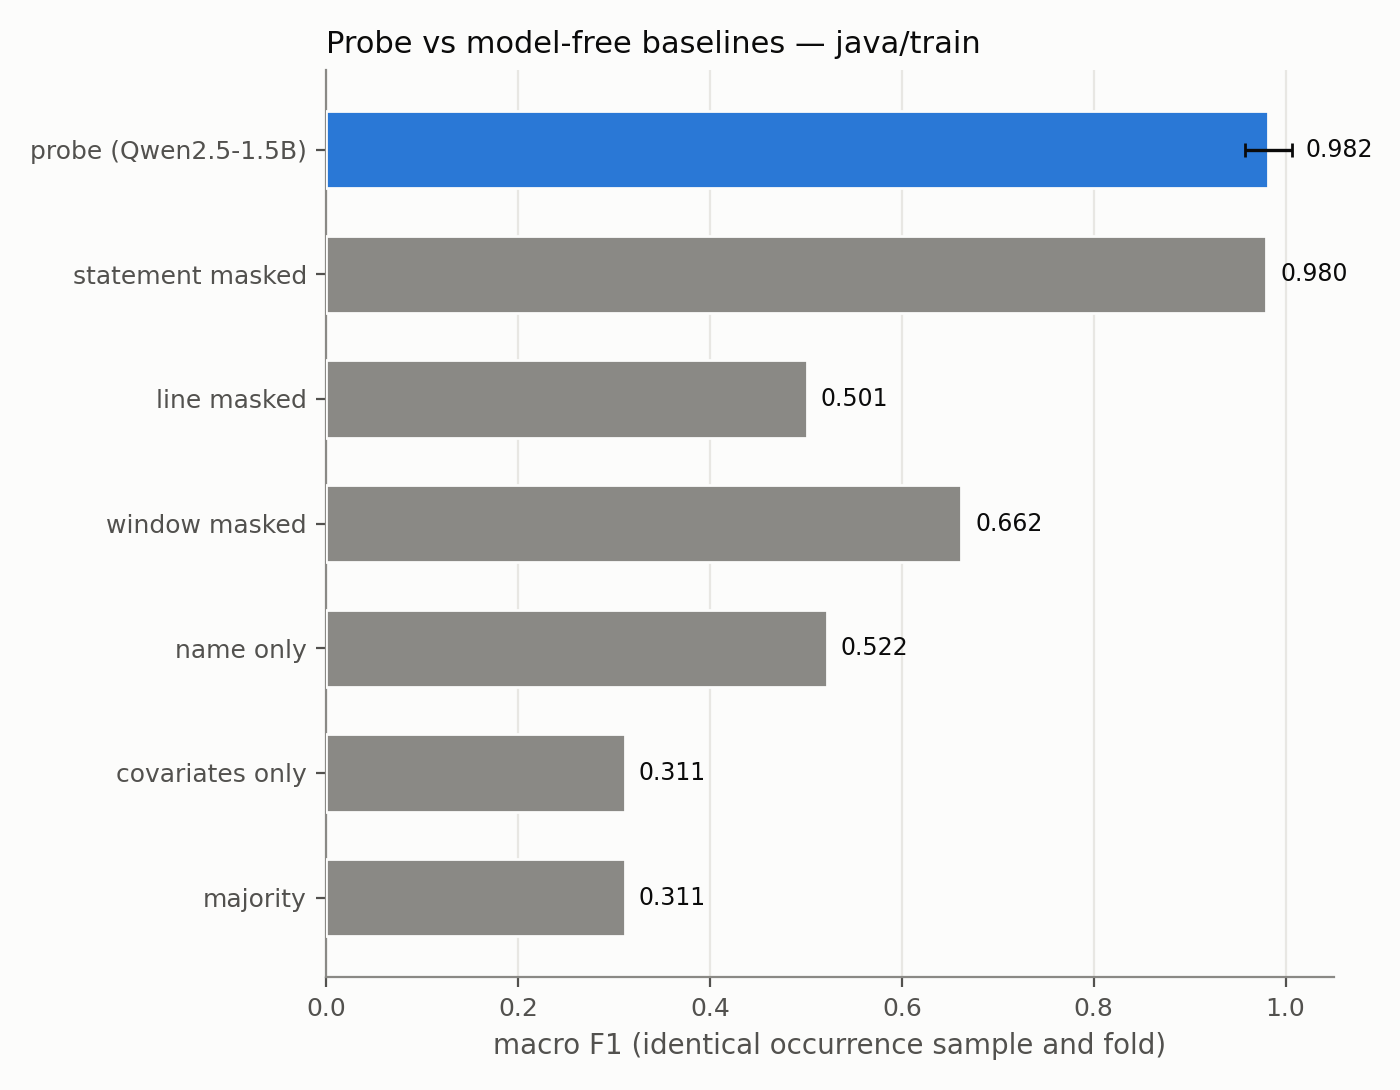
\includegraphics[width=\linewidth]{../results/boolean/probe_vs_baselines_java_train_qwen2515b.png}
\caption{Java}
\label{fig:boolean-probe-java-qwen2515b}
\end{subfigure}\hfill
\begin{subfigure}{0.49\linewidth}\centering
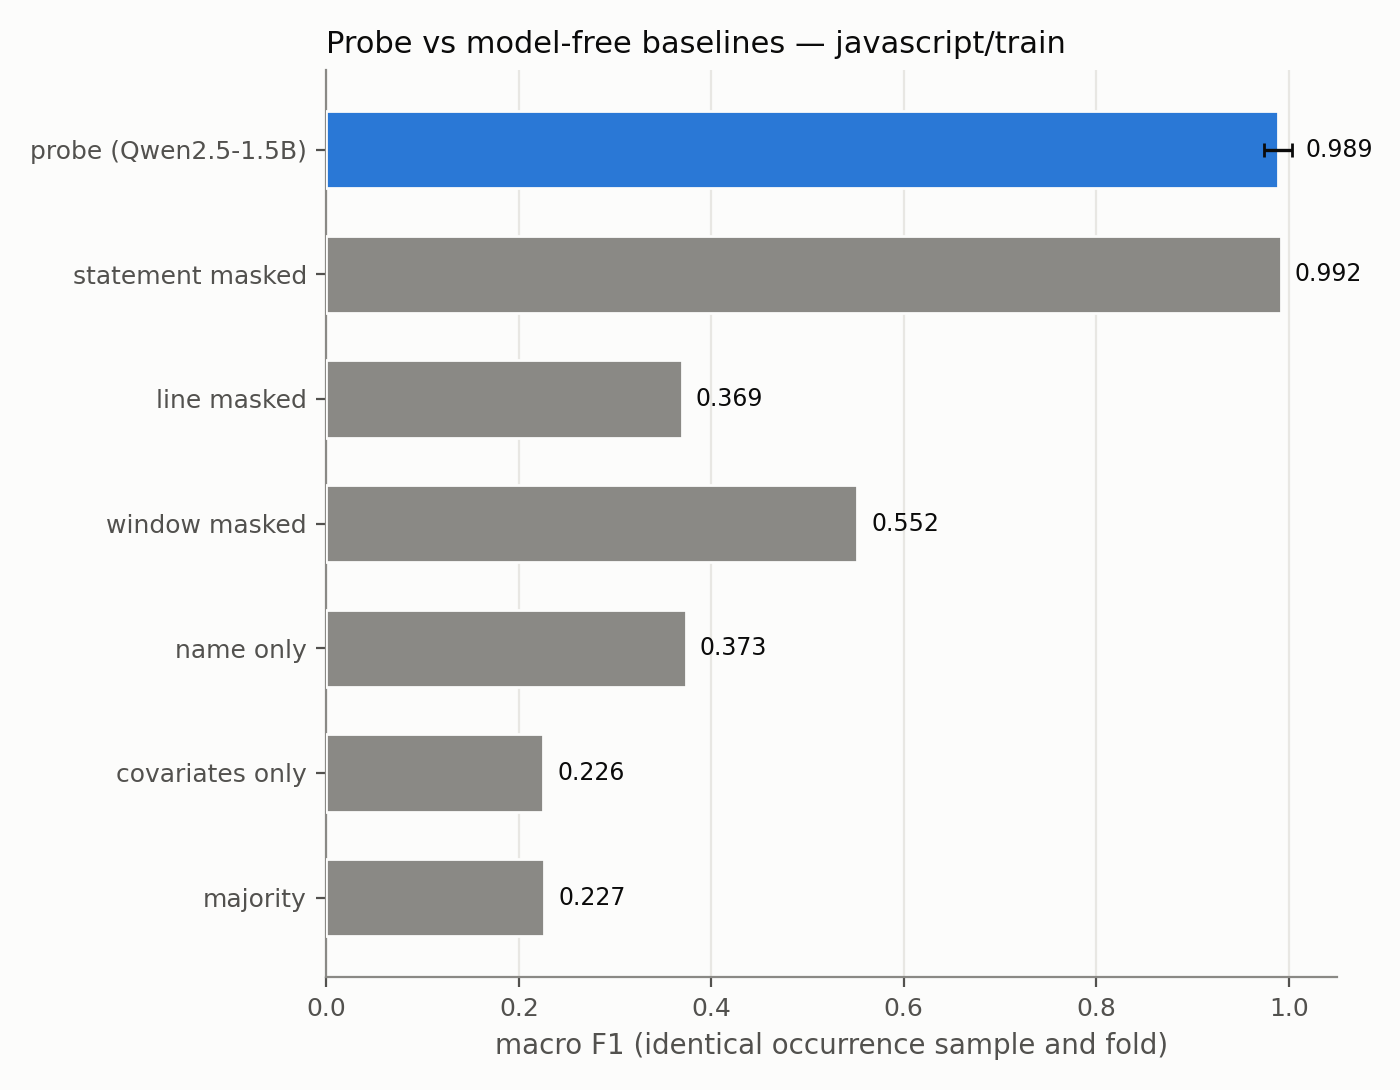
\includegraphics[width=\linewidth]{../results/boolean/probe_vs_baselines_javascript_train_qwen2515b.png}
\caption{JavaScript}
\label{fig:boolean-probe-javascript-qwen2515b}
\end{subfigure}
\begin{subfigure}{0.49\linewidth}\centering
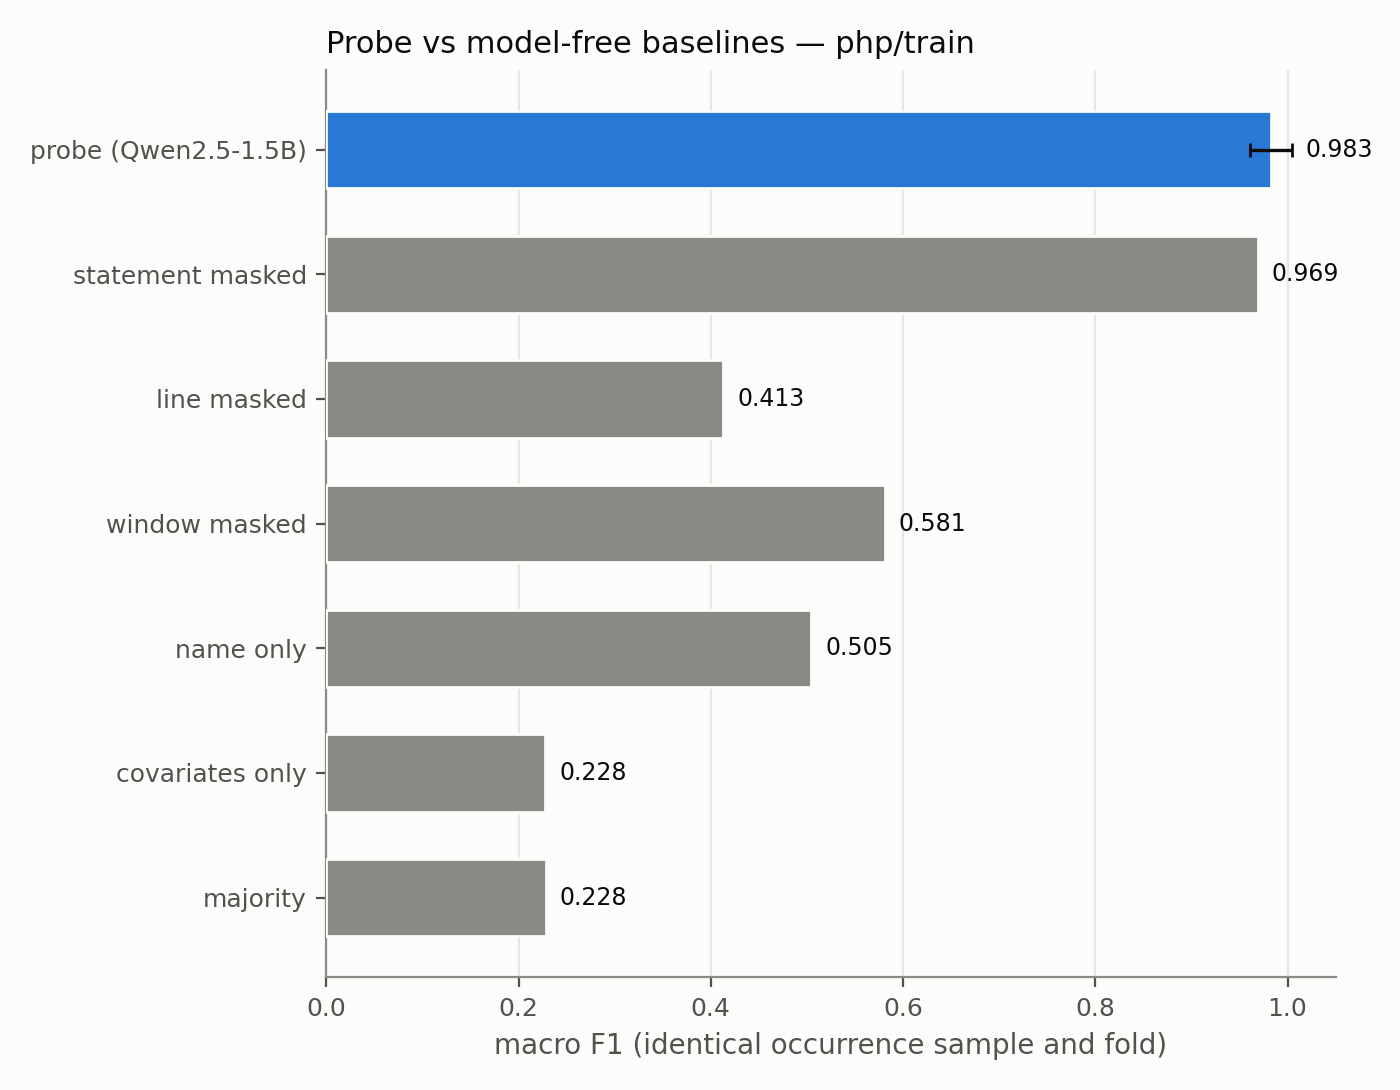
\includegraphics[width=\linewidth]{../results/boolean/probe_vs_baselines_php_train_qwen2515b.png}
\caption{PHP}
\label{fig:boolean-probe-php-qwen2515b}
\end{subfigure}\hfill
\begin{subfigure}{0.49\linewidth}\centering
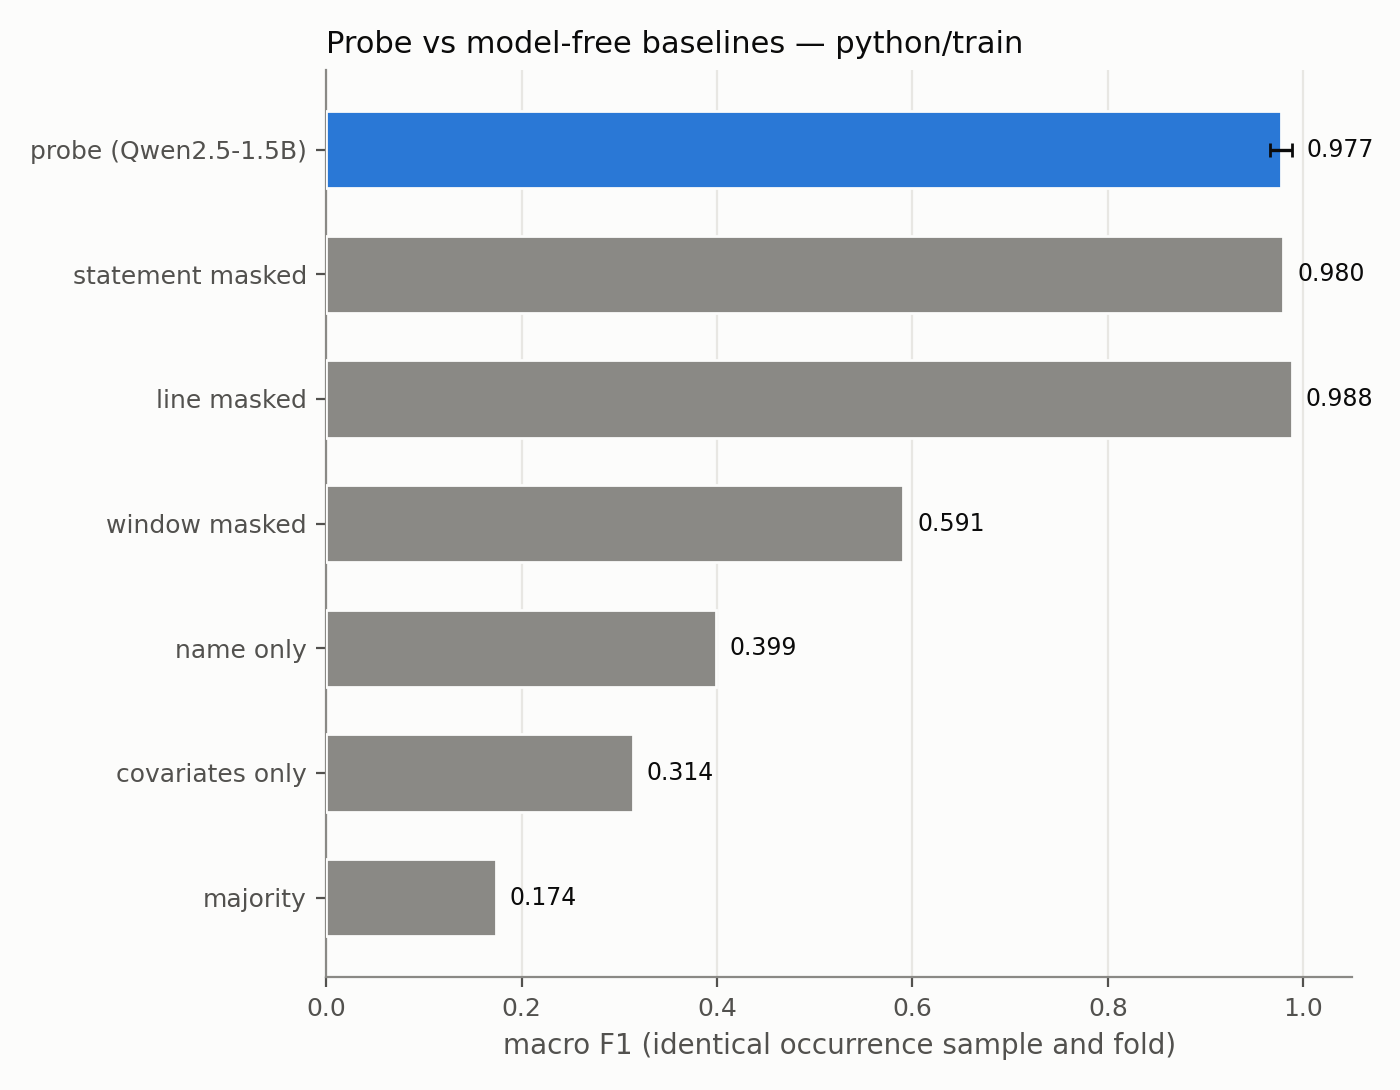
\includegraphics[width=\linewidth]{../results/boolean/probe_vs_baselines_python_train_qwen2515b.png}
\caption{Python}
\label{fig:boolean-probe-python-qwen2515b}
\end{subfigure}
\caption{Boolean probe and model-free baselines for Qwen2.5-1.5B across the four committed languages.}
\label{fig:boolean-gallery-probe-qwen2515b}
\end{figure}
\begin{figure}[htbp]\centering
\begin{subfigure}{0.49\linewidth}\centering
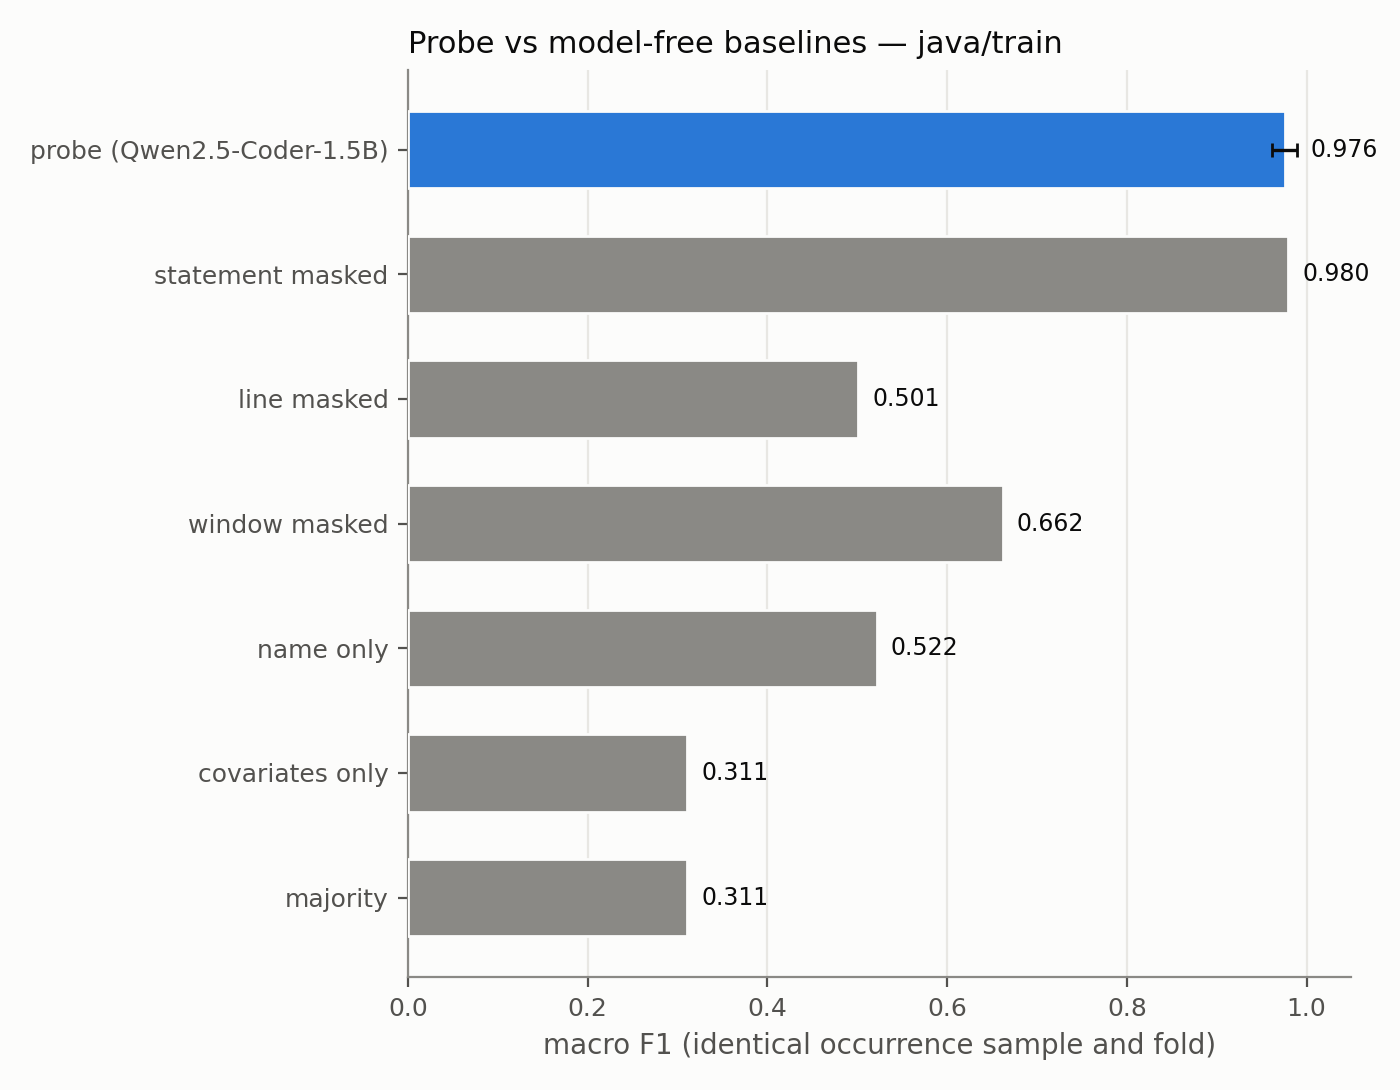
\includegraphics[width=\linewidth]{../results/boolean/probe_vs_baselines_java_train_qwen25coder15b.png}
\caption{Java}
\label{fig:boolean-probe-java-qwen25coder15b}
\end{subfigure}\hfill
\begin{subfigure}{0.49\linewidth}\centering
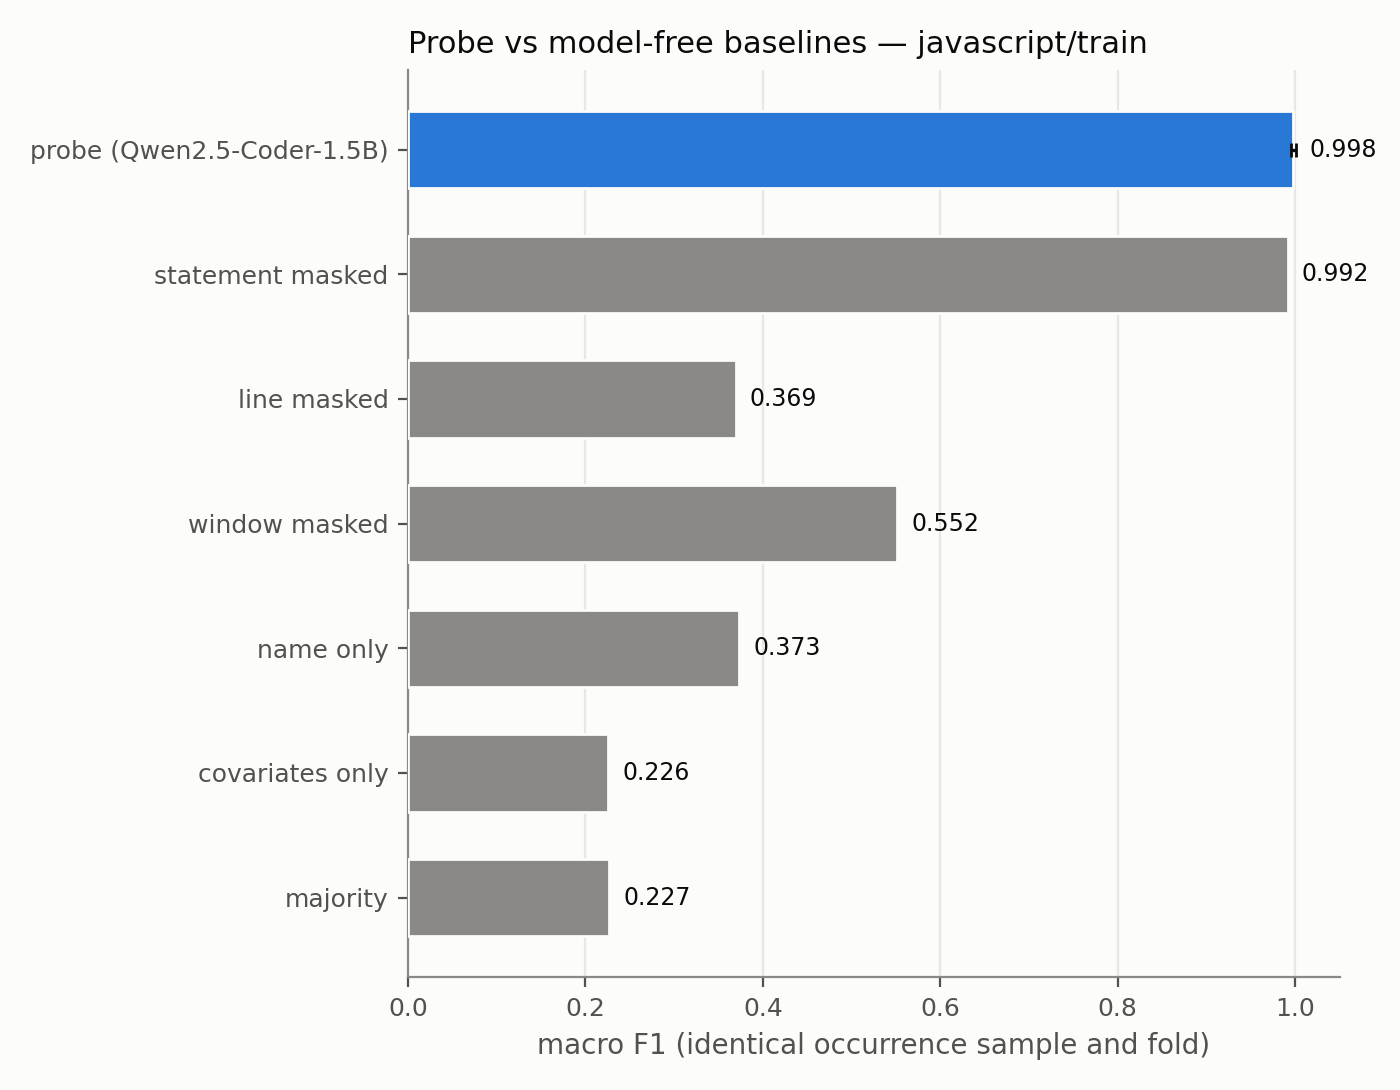
\includegraphics[width=\linewidth]{../results/boolean/probe_vs_baselines_javascript_train_qwen25coder15b.png}
\caption{JavaScript}
\label{fig:boolean-probe-javascript-qwen25coder15b}
\end{subfigure}
\begin{subfigure}{0.49\linewidth}\centering
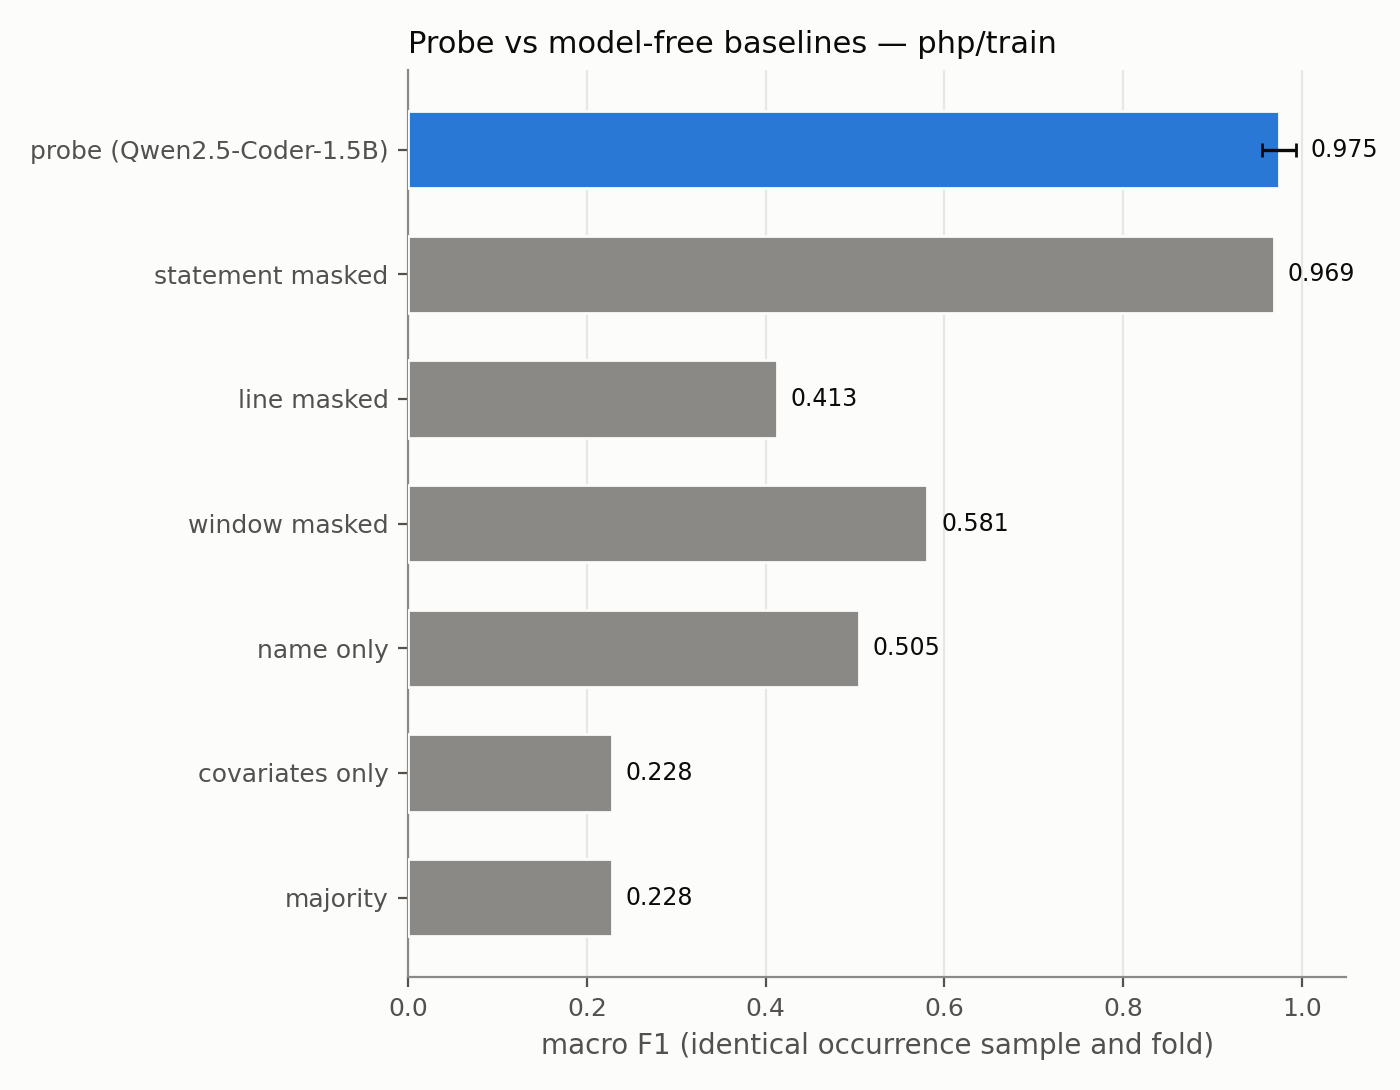
\includegraphics[width=\linewidth]{../results/boolean/probe_vs_baselines_php_train_qwen25coder15b.png}
\caption{PHP}
\label{fig:boolean-probe-php-qwen25coder15b}
\end{subfigure}\hfill
\begin{subfigure}{0.49\linewidth}\centering
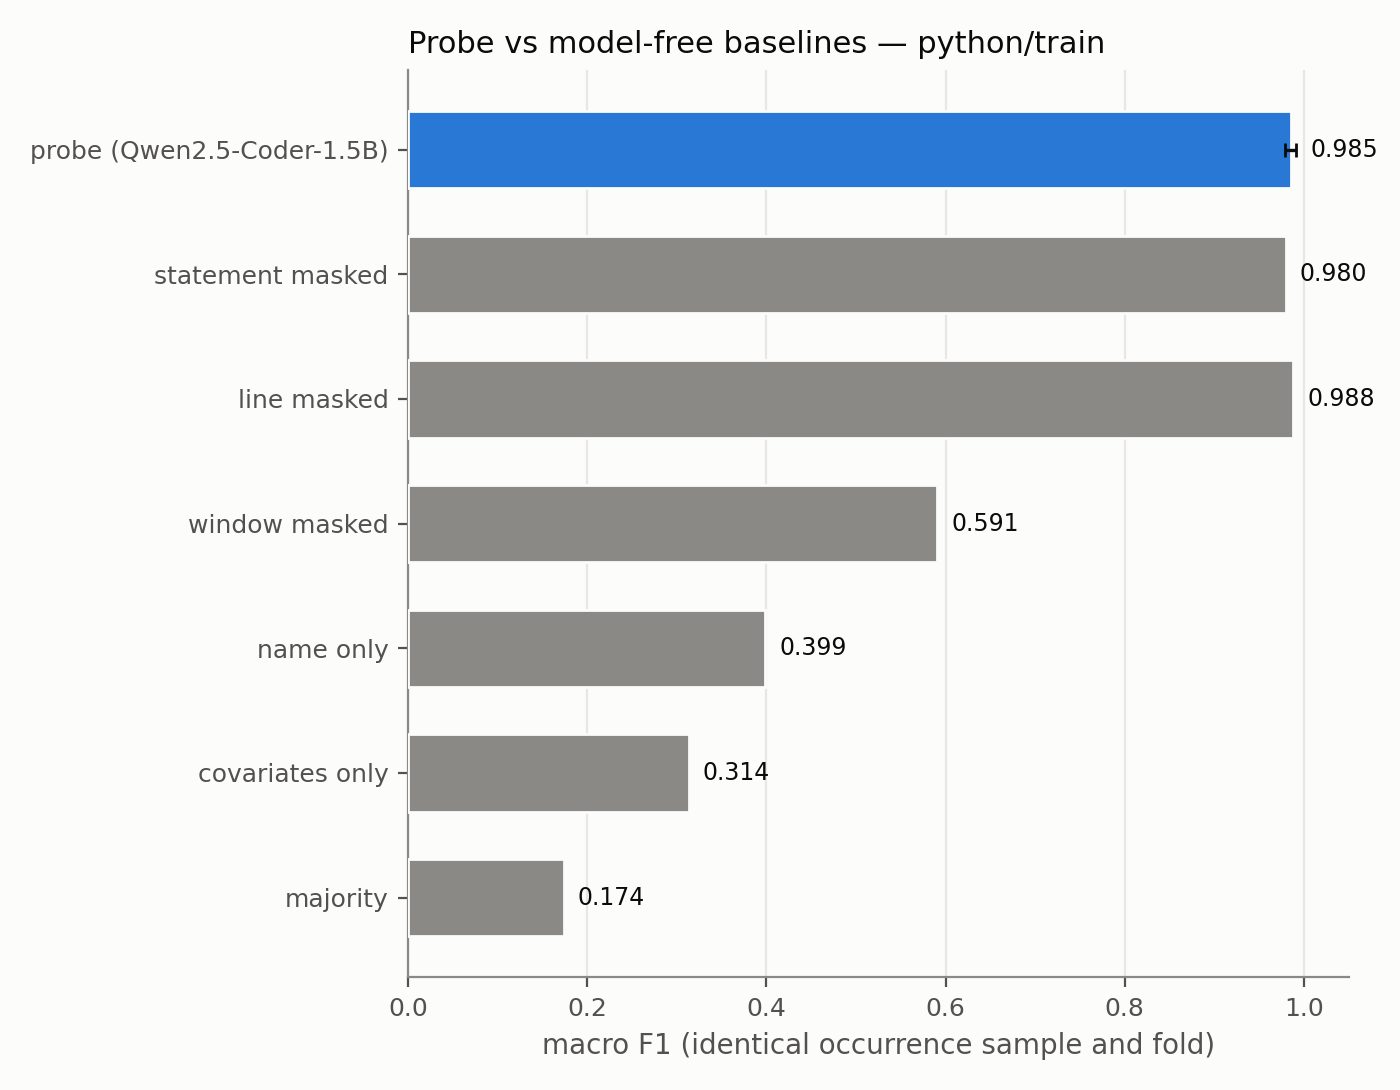
\includegraphics[width=\linewidth]{../results/boolean/probe_vs_baselines_python_train_qwen25coder15b.png}
\caption{Python}
\label{fig:boolean-probe-python-qwen25coder15b}
\end{subfigure}
\caption{Boolean probe and model-free baselines for Qwen2.5-Coder-1.5B across the four committed languages.}
\label{fig:boolean-gallery-probe-qwen25coder15b}
\end{figure}
\begin{figure}[htbp]\centering
\begin{subfigure}{0.49\linewidth}\centering
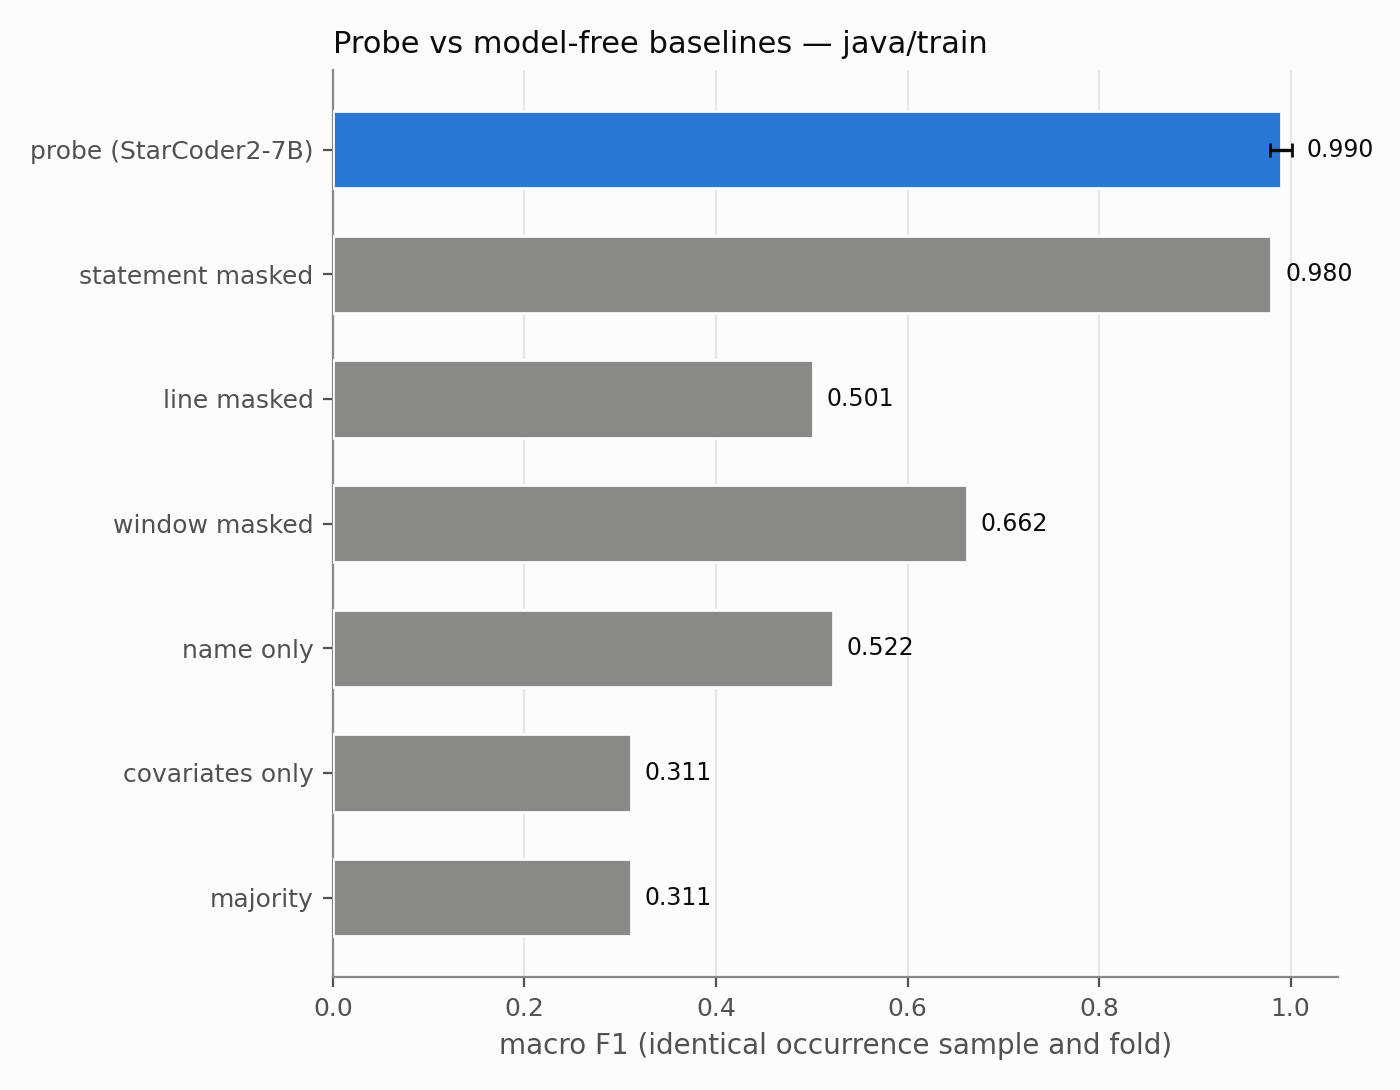
\includegraphics[width=\linewidth]{../results/boolean/probe_vs_baselines_java_train_starcoder27b.png}
\caption{Java}
\label{fig:boolean-probe-java-starcoder27b}
\end{subfigure}\hfill
\begin{subfigure}{0.49\linewidth}\centering
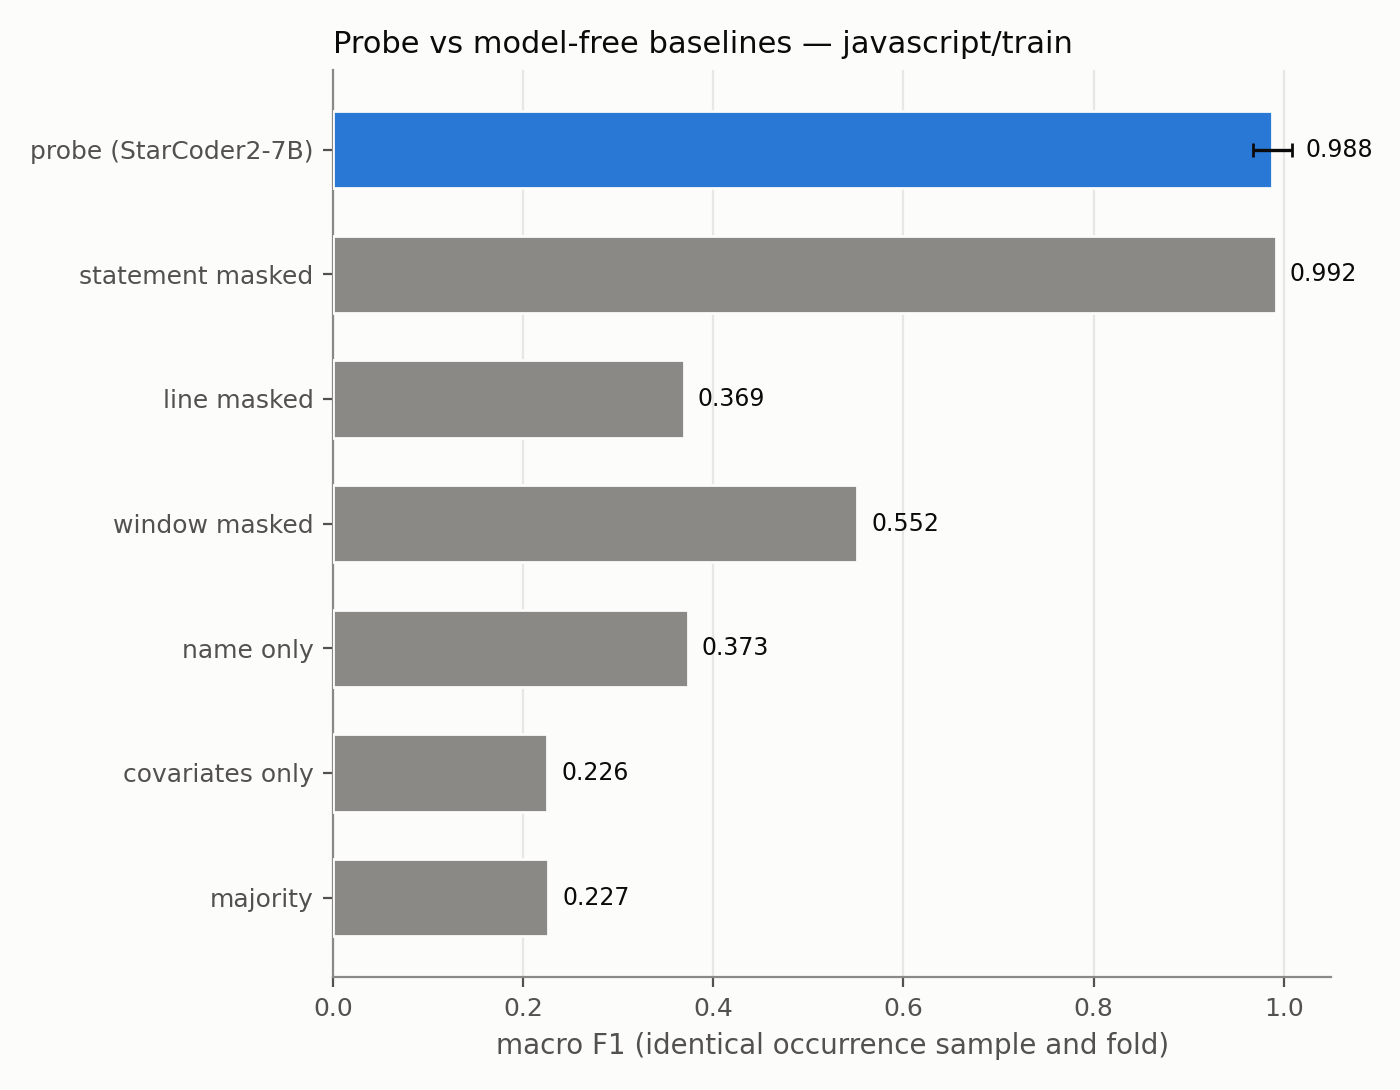
\includegraphics[width=\linewidth]{../results/boolean/probe_vs_baselines_javascript_train_starcoder27b.png}
\caption{JavaScript}
\label{fig:boolean-probe-javascript-starcoder27b}
\end{subfigure}
\begin{subfigure}{0.49\linewidth}\centering
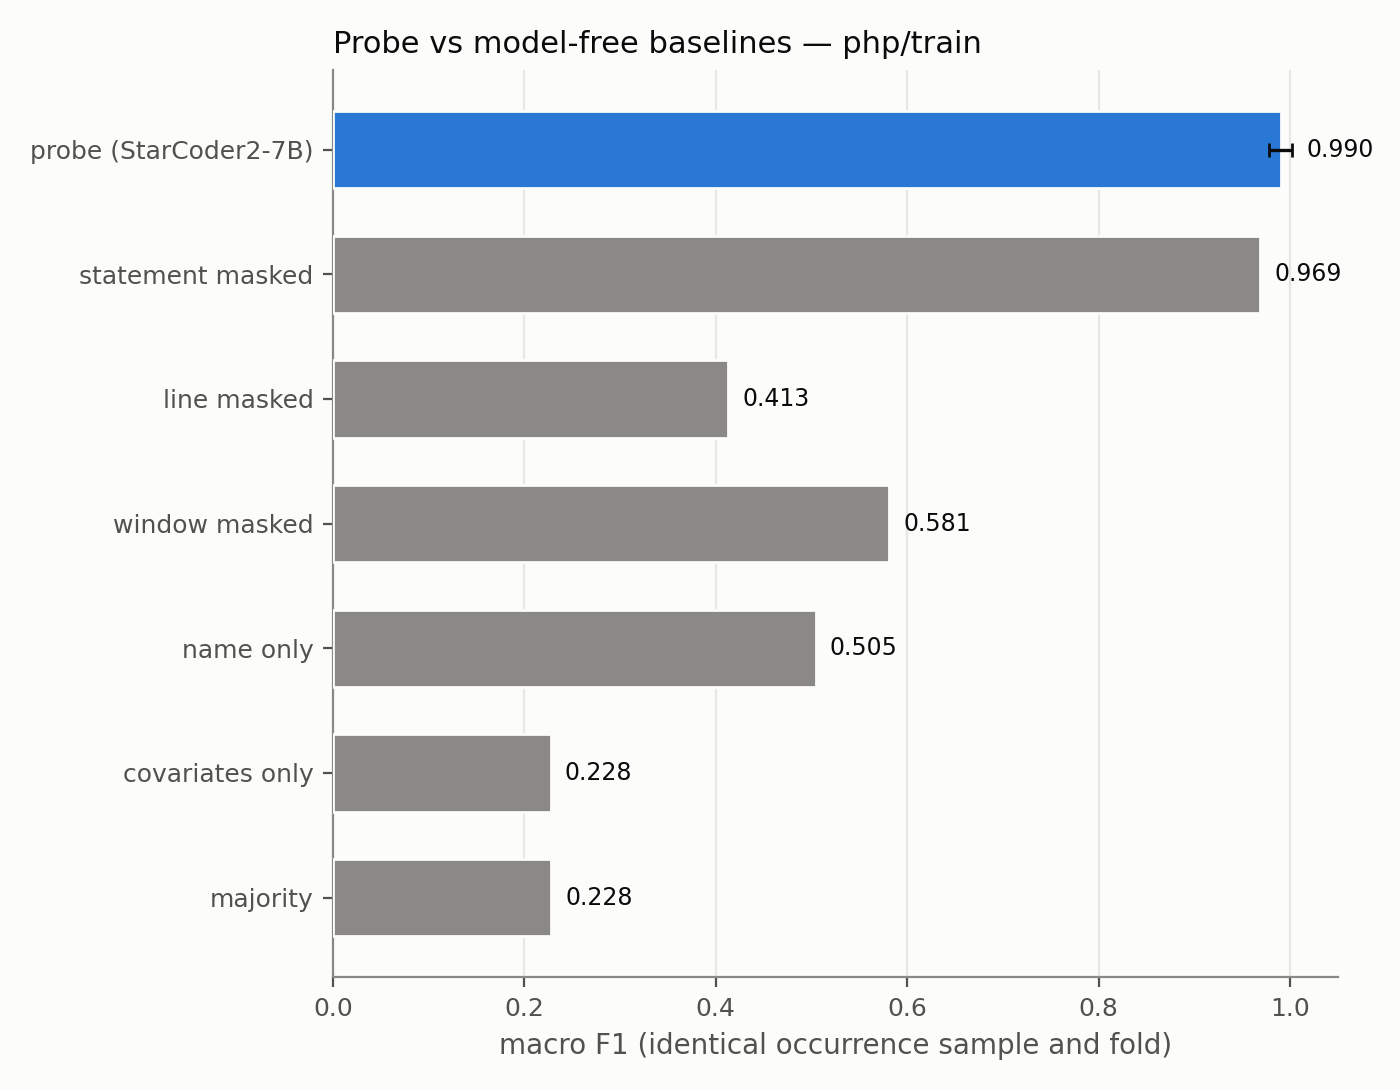
\includegraphics[width=\linewidth]{../results/boolean/probe_vs_baselines_php_train_starcoder27b.png}
\caption{PHP}
\label{fig:boolean-probe-php-starcoder27b}
\end{subfigure}\hfill
\begin{subfigure}{0.49\linewidth}\centering
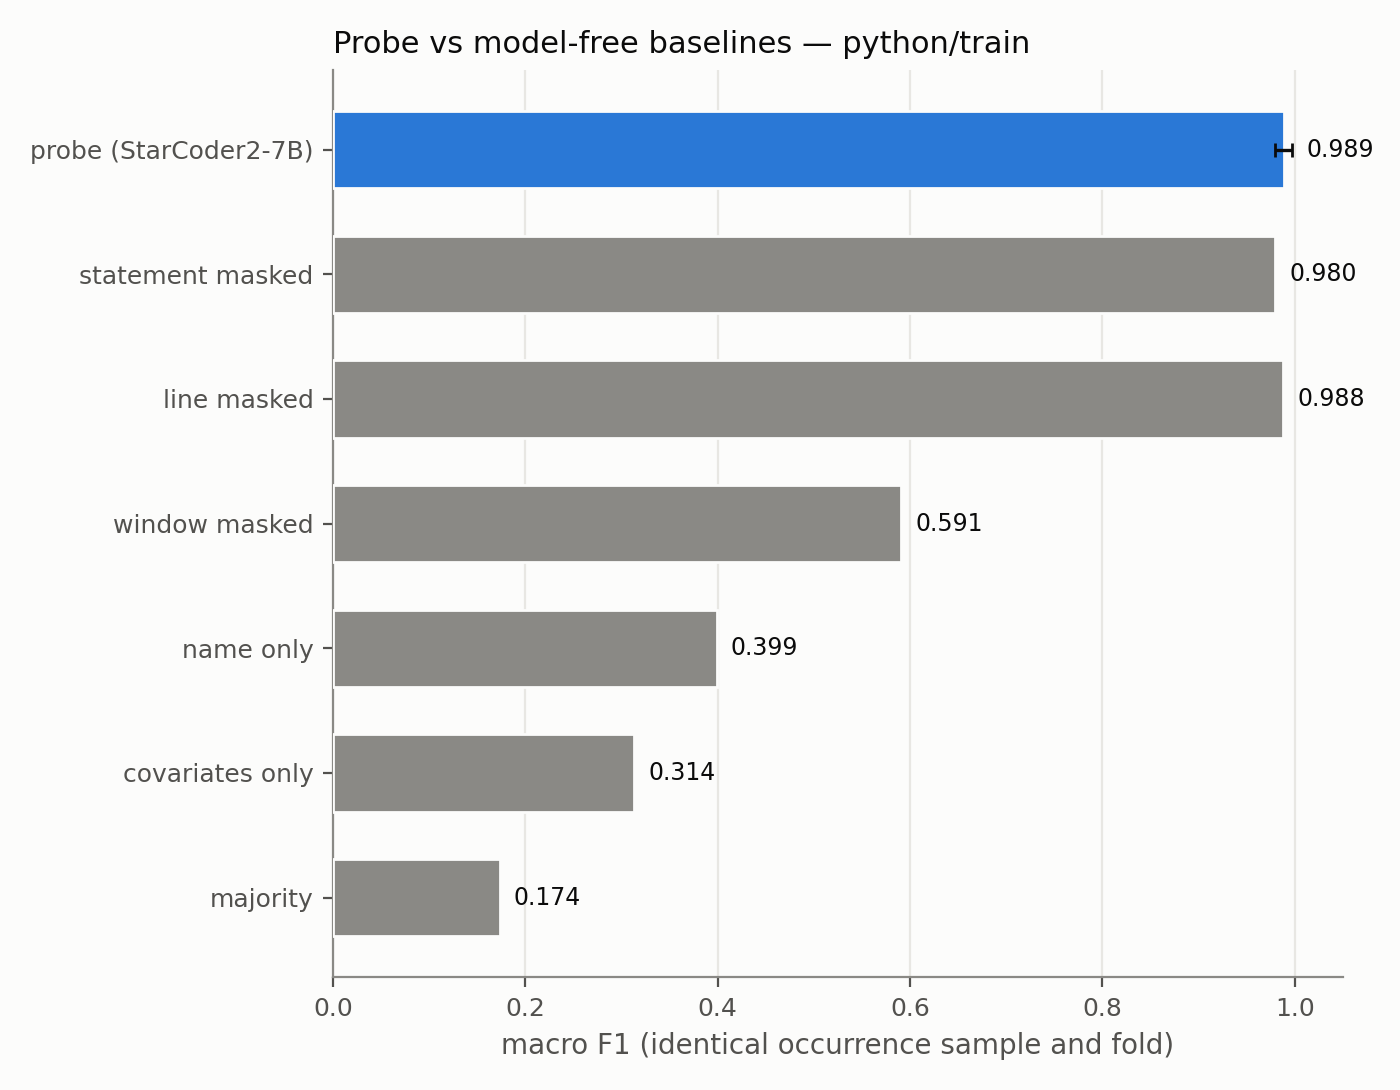
\includegraphics[width=\linewidth]{../results/boolean/probe_vs_baselines_python_train_starcoder27b.png}
\caption{Python}
\label{fig:boolean-probe-python-starcoder27b}
\end{subfigure}
\caption{Boolean probe and model-free baselines for StarCoder2-7B across the four committed languages.}
\label{fig:boolean-gallery-probe-starcoder27b}
\end{figure}
\begin{figure}[htbp]\centering
\begin{subfigure}{0.49\linewidth}\centering
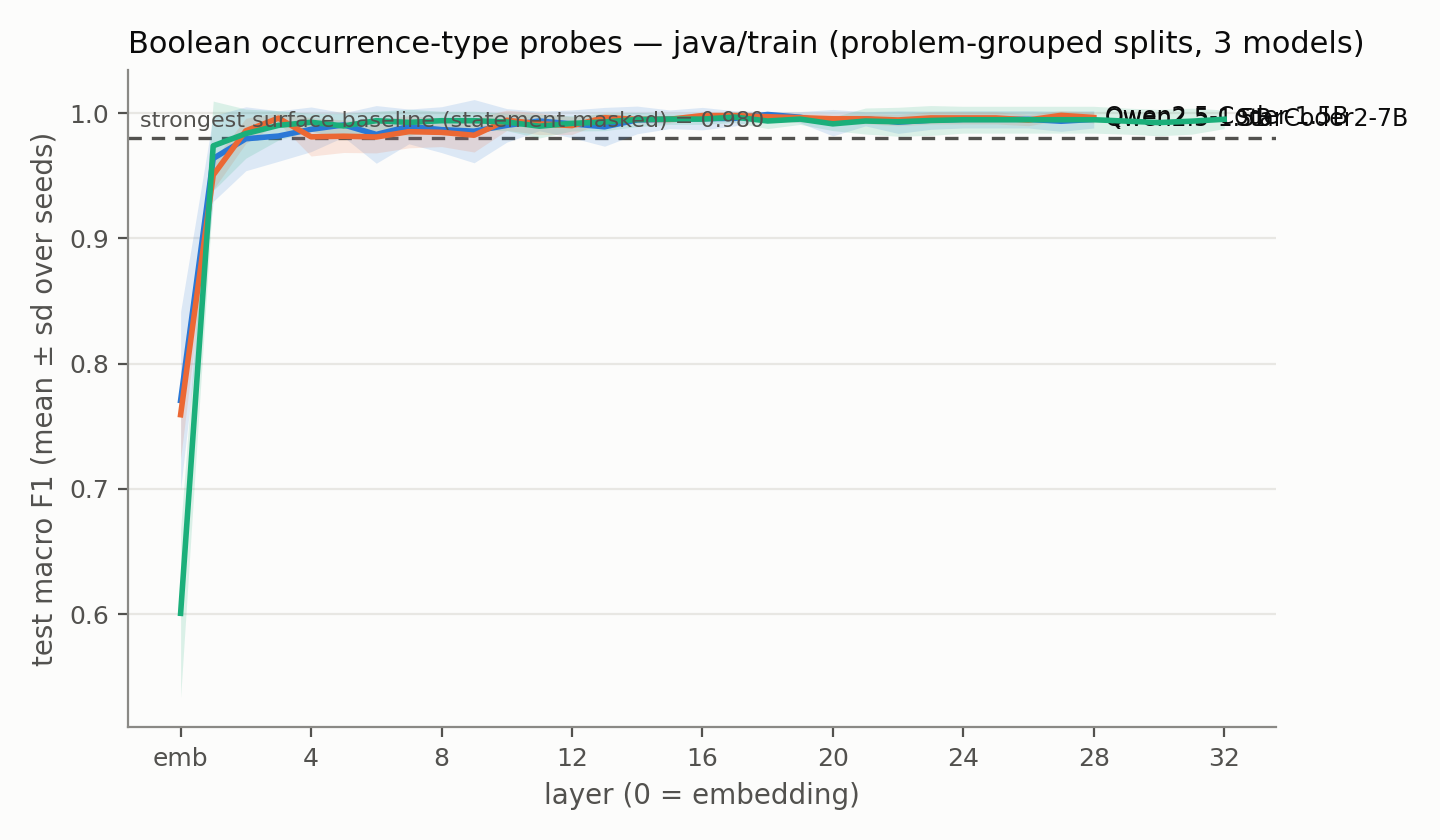
\includegraphics[width=\linewidth]{../results/boolean/layer_curves_java_train.png}
\caption{Java}
\label{fig:boolean-layers-java}
\end{subfigure}\hfill
\begin{subfigure}{0.49\linewidth}\centering
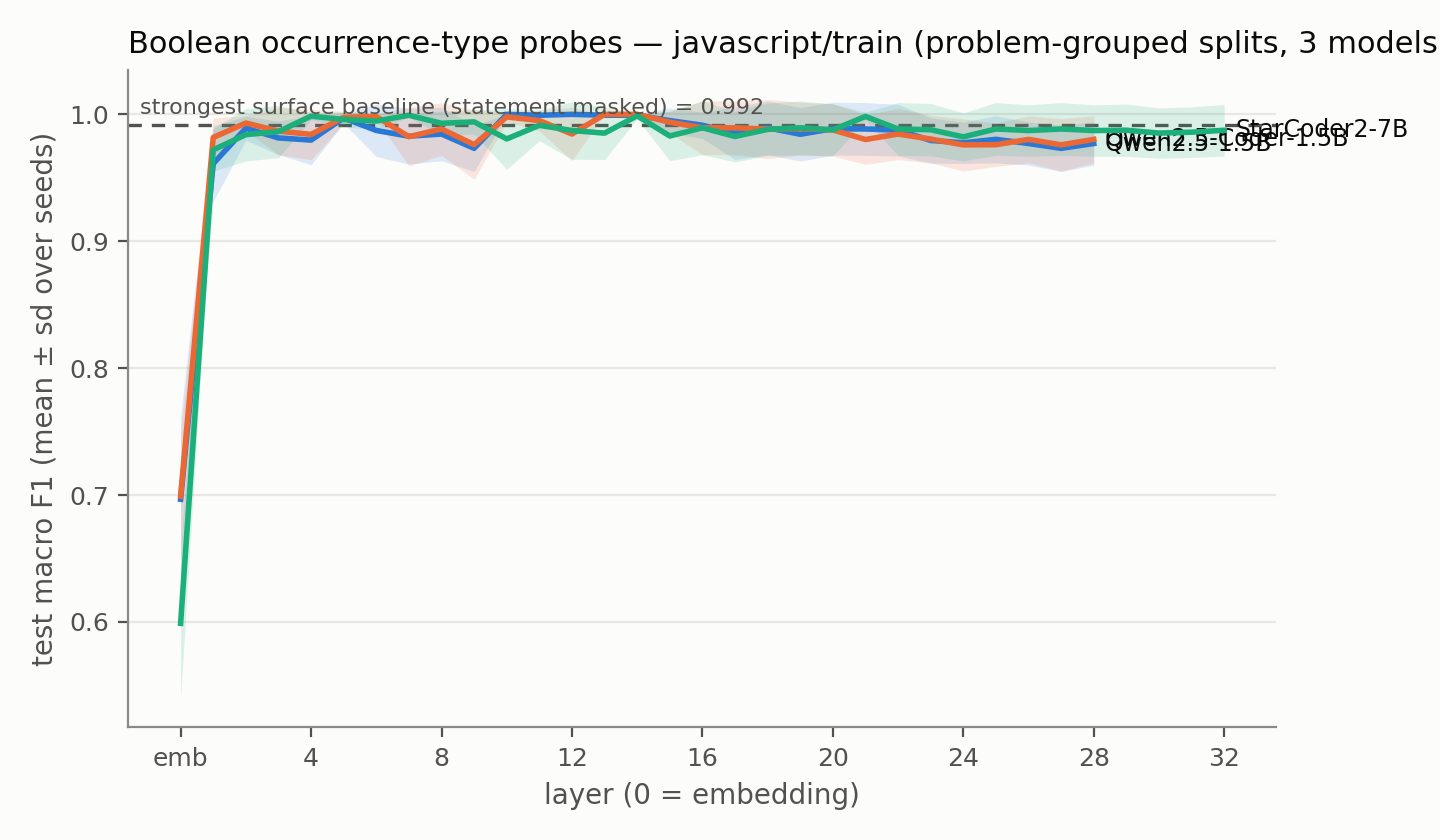
\includegraphics[width=\linewidth]{../results/boolean/layer_curves_javascript_train.png}
\caption{JavaScript}
\label{fig:boolean-layers-javascript}
\end{subfigure}
\begin{subfigure}{0.49\linewidth}\centering
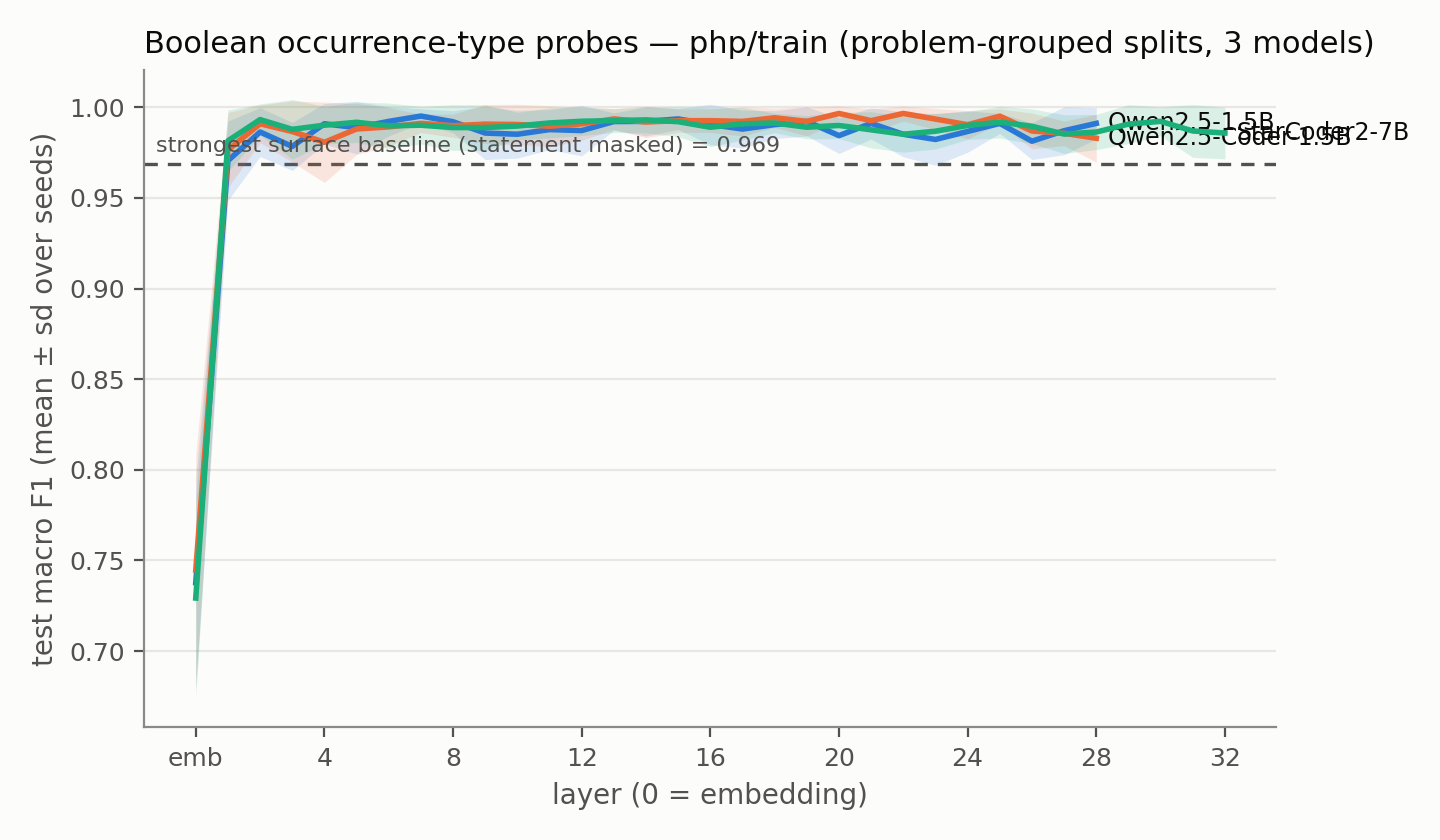
\includegraphics[width=\linewidth]{../results/boolean/layer_curves_php_train.png}
\caption{PHP}
\label{fig:boolean-layers-php}
\end{subfigure}\hfill
\begin{subfigure}{0.49\linewidth}\centering
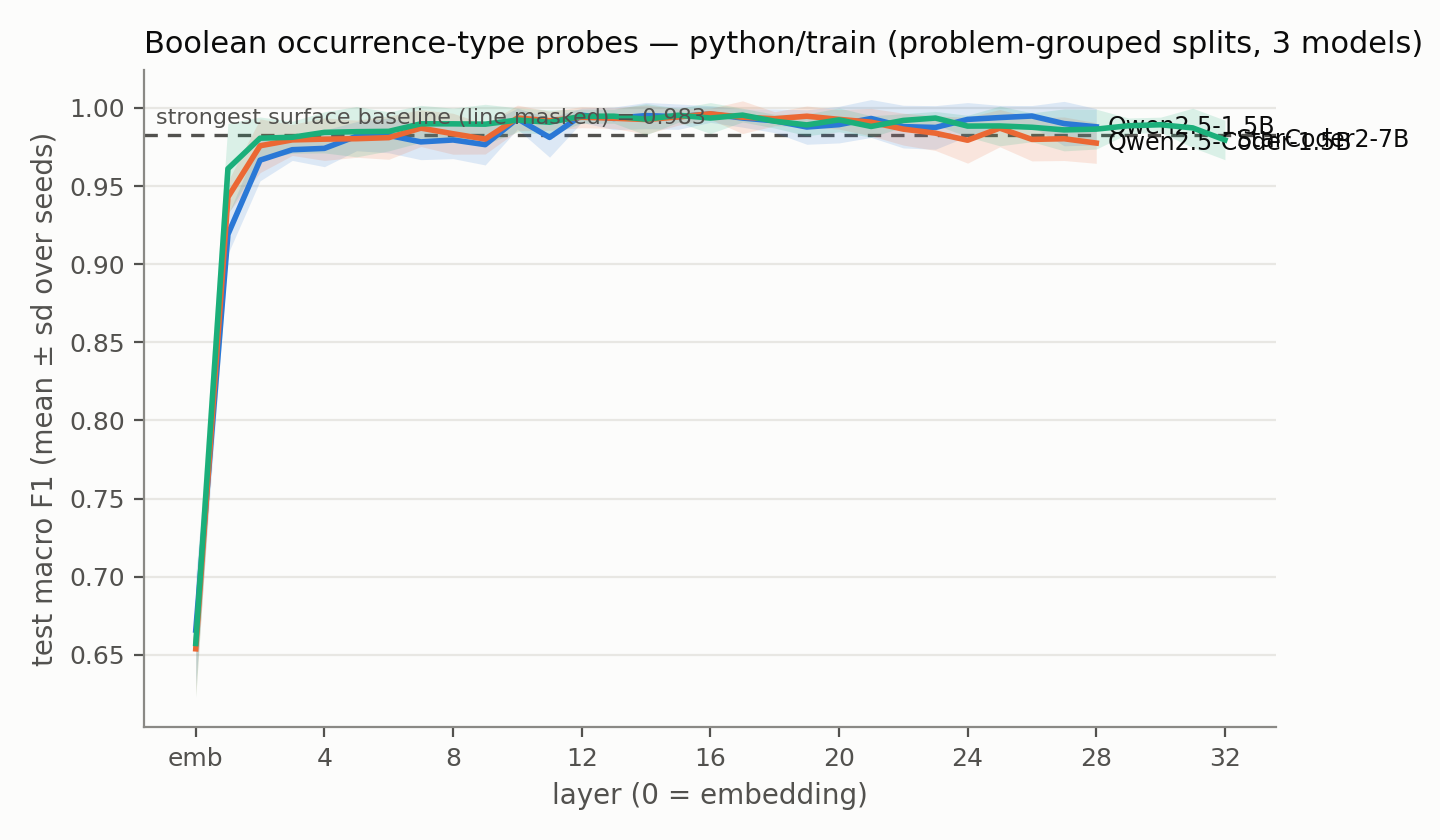
\includegraphics[width=\linewidth]{../results/boolean/layer_curves_python_train.png}
\caption{Python}
\label{fig:boolean-layers-python}
\end{subfigure}
\caption{Boolean probe layer curves per language across the three models.}
\label{fig:boolean-gallery-layers}
\end{figure}
\begin{figure}[htbp]\centering
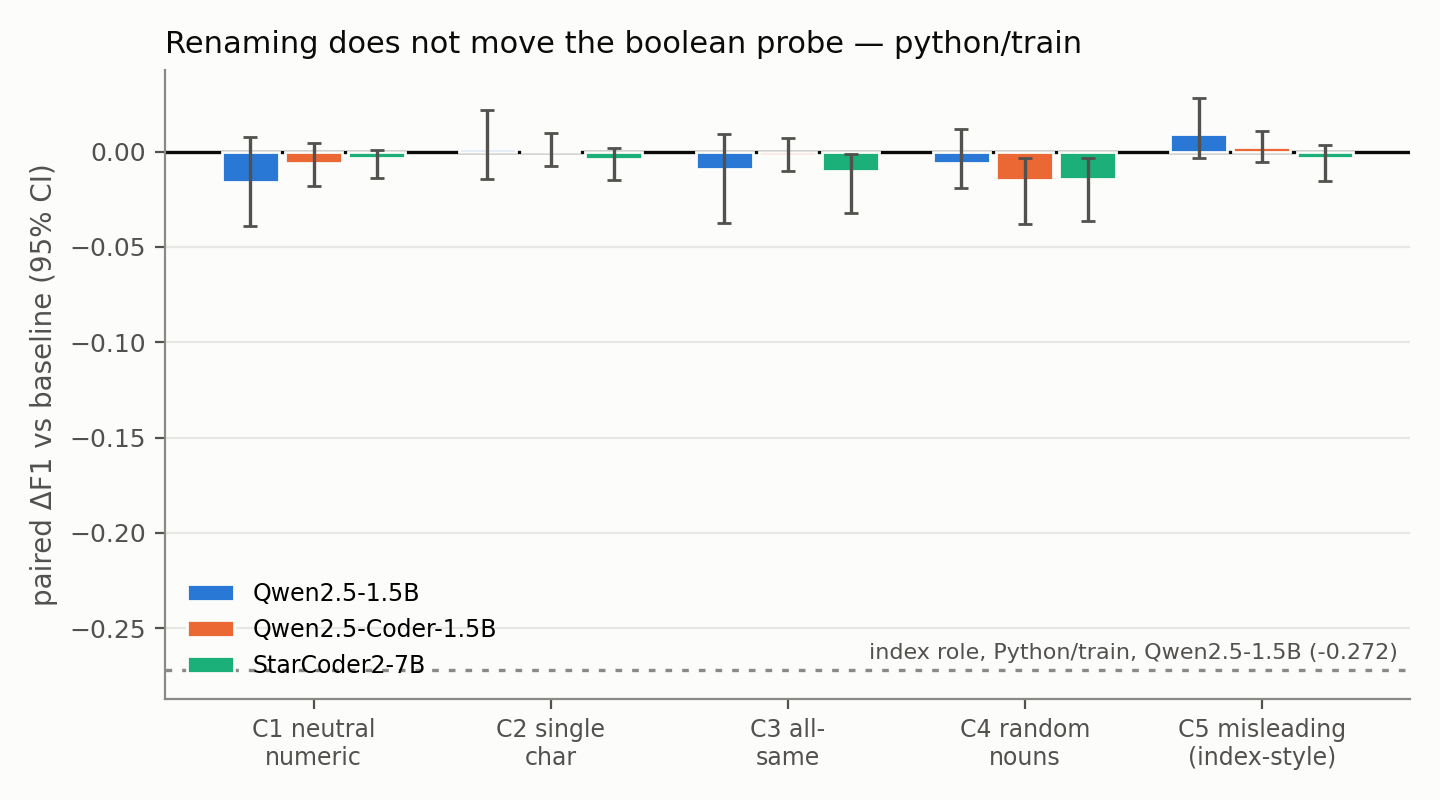
\includegraphics[width=0.78\linewidth]{../results/boolean/renaming_deltas_python_train.png}
\caption{Problem-paired boolean refit-performance deltas on Python. No corresponding committed renaming run exists for other languages.}
\label{fig:boolean-renaming-python}
\end{figure}

\begin{table}[htbp]\centering\small
\caption{Complete class/structure perturbation results under the shared five-seed protocol. Each condition refits a probe and selects its own layer on validation data, so cross-condition deltas do not test a fixed direction.}
\label{tab:class-full}
\resizebox{\ifdim\width>\linewidth\linewidth\else\width\fi}{!}{%
\begin{tabular}{llrrrrrr}
\toprule
model & strategy & layer & F1 & 95\% CI & control F1 & selectivity & $\Delta$ \\
\midrule
Qwen2.5-1.5B & baseline & L18 & 0.979 & [0.967, 0.987] & 0.427 & +0.552 & N/A \\
Qwen2.5-1.5B & random\_nouns & L20 & 0.986 & [0.976, 0.992] & 0.426 & +0.560 & +0.007 \\
Qwen2.5-1.5B & single\_chars & L11 & 0.957 & [0.936, 0.969] & 0.423 & +0.534 & -0.022 \\
Qwen2.5-1.5B & all\_same & L0 & 1.000 & [1.000, 1.000] & 0.440 & +0.560 & +0.021 \\
Qwen2.5-1.5B & numeric\_vars & L21 & 0.965 & [0.952, 0.972] & 0.422 & +0.543 & -0.014 \\
Qwen2.5-1.5B & misleading\_class\_struct & L7 & 0.976 & [0.962, 0.982] & 0.416 & +0.559 & -0.004 \\
Qwen2.5-Coder-1.5B & baseline & L8 & 0.982 & [0.969, 0.989] & 0.429 & +0.553 & N/A \\
Qwen2.5-Coder-1.5B & random\_nouns & L19 & 0.978 & [0.965, 0.985] & 0.427 & +0.551 & -0.004 \\
Qwen2.5-Coder-1.5B & single\_chars & L7 & 0.956 & [0.936, 0.967] & 0.423 & +0.533 & -0.026 \\
Qwen2.5-Coder-1.5B & all\_same & L0 & 1.000 & [1.000, 1.000] & 0.440 & +0.560 & +0.018 \\
Qwen2.5-Coder-1.5B & numeric\_vars & L21 & 0.968 & [0.955, 0.975] & 0.424 & +0.544 & -0.014 \\
Qwen2.5-Coder-1.5B & misleading\_class\_struct & L7 & 0.978 & [0.967, 0.984] & 0.415 & +0.562 & -0.004 \\
StarCoder2-7B & baseline & L5 & 0.981 & [0.967, 0.990] & 0.478 & +0.503 & N/A \\
StarCoder2-7B & random\_nouns & L6 & 0.976 & [0.962, 0.983] & 0.466 & +0.510 & -0.006 \\
StarCoder2-7B & single\_chars & L4 & 0.957 & [0.921, 0.971] & 0.475 & +0.482 & -0.025 \\
StarCoder2-7B & all\_same & L0 & 1.000 & [1.000, 1.000] & 0.445 & +0.555 & +0.019 \\
StarCoder2-7B & numeric\_vars & L23 & 0.968 & [0.956, 0.975] & 0.451 & +0.517 & -0.013 \\
StarCoder2-7B & misleading\_class\_struct & L5 & 0.985 & [0.976, 0.990] & 0.467 & +0.518 & +0.004 \\
\bottomrule
\end{tabular}}
\end{table}

\begin{table}[htbp]\centering\small
\caption{Class/structure cross-language results. Transfer uses the Python-selected layer without a shared source-target problem partition. In-domain layers are selected separately. Only languages present in the committed exports are shown.}
\label{tab:class-crosslang}
\resizebox{\ifdim\width>\linewidth\linewidth\else\width\fi}{!}{%
\begin{tabular}{llrrrrrr}
\toprule
model & language & programs & in-domain layer & in-domain F1 & transfer accuracy & transfer F1 \\
\midrule
Qwen2.5-1.5B & Python & 400 & L18 & 0.979 & N/A & N/A \\
Qwen2.5-1.5B & C++ & 606 & L10 & 0.991 & 0.993 & 0.933 \\
Qwen2.5-1.5B & JavaScript & 285 & L5 & 0.987 & 0.998 & 0.957 \\
Qwen2.5-1.5B & C & 97 & L8 & 0.986 & 0.984 & 0.886 \\
Qwen2.5-Coder-1.5B & Python & 400 & L8 & 0.982 & N/A & N/A \\
Qwen2.5-Coder-1.5B & C++ & 606 & L8 & 0.988 & 0.991 & 0.918 \\
Qwen2.5-Coder-1.5B & JavaScript & 285 & L6 & 0.985 & 0.996 & 0.913 \\
Qwen2.5-Coder-1.5B & C & 97 & L20 & 0.980 & 0.983 & 0.885 \\
StarCoder2-7B & Python & 400 & L5 & 0.981 & N/A & N/A \\
StarCoder2-7B & C++ & 606 & L5 & 0.992 & 0.996 & 0.965 \\
StarCoder2-7B & JavaScript & 285 & L3 & 0.989 & 0.999 & 0.980 \\
StarCoder2-7B & C & 97 & L5 & 0.986 & 0.987 & 0.906 \\
\bottomrule
\end{tabular}}
\end{table}

\begin{table}[htbp]\centering\small
\caption{Layerwise class/structure robustness summaries. The F1 range is taken over all committed layers. Maximum cosine similarity is measured against the baseline activation direction for each renamed condition.}
\label{tab:class-layerwise}
\resizebox{\ifdim\width>\linewidth\linewidth\else\width\fi}{!}{%
\begin{tabular}{llrrrr}
\toprule
model & strategy & minimum F1 & maximum F1 (layer) & maximum cosine (layer) \\
\midrule
Qwen2.5-1.5B & all\_same & 0.999 & 1.000 (L0) & 0.105 (L11) \\
Qwen2.5-1.5B & baseline & 0.806 & 0.983 (L18) & N/A \\
Qwen2.5-1.5B & misleading\_class\_struct & 0.708 & 0.980 (L7) & 0.311 (L15) \\
Qwen2.5-1.5B & numeric\_vars & 0.445 & 0.966 (L21) & 0.329 (L22) \\
Qwen2.5-1.5B & random\_nouns & 0.529 & 0.989 (L15) & 0.493 (L26) \\
Qwen2.5-1.5B & single\_chars & 0.530 & 0.965 (L7) & 0.392 (L15) \\
Qwen2.5-Coder-1.5B & all\_same & 0.999 & 1.000 (L0) & 0.126 (L28) \\
Qwen2.5-Coder-1.5B & baseline & 0.807 & 0.985 (L7) & N/A \\
Qwen2.5-Coder-1.5B & misleading\_class\_struct & 0.708 & 0.978 (L7) & 0.324 (L7) \\
Qwen2.5-Coder-1.5B & numeric\_vars & 0.445 & 0.969 (L24) & 0.352 (L22) \\
Qwen2.5-Coder-1.5B & random\_nouns & 0.530 & 0.983 (L23) & 0.464 (L19) \\
Qwen2.5-Coder-1.5B & single\_chars & 0.530 & 0.959 (L7) & 0.415 (L15) \\
StarCoder2-7B & all\_same & 0.999 & 1.000 (L0) & 0.101 (L21) \\
StarCoder2-7B & baseline & 0.763 & 0.984 (L6) & N/A \\
StarCoder2-7B & misleading\_class\_struct & 0.717 & 0.985 (L3) & 0.387 (L3) \\
StarCoder2-7B & numeric\_vars & 0.443 & 0.971 (L26) & 0.369 (L22) \\
StarCoder2-7B & random\_nouns & 0.502 & 0.979 (L8) & 0.511 (L3) \\
StarCoder2-7B & single\_chars & 0.529 & 0.962 (L3) & 0.467 (L6) \\
\bottomrule
\end{tabular}}
\end{table}

\begin{table}[htbp]\centering\small
\caption{Complete iterator perturbation results under the shared five-seed protocol. Each condition refits a probe and selects its own layer on validation data. Role-conditioned and non-bijective strategies are confounded diagnostics rather than robustness tests.}
\label{tab:iterator-full}
\resizebox{\ifdim\width>\linewidth\linewidth\else\width\fi}{!}{%
\begin{tabular}{llrrrrrr}
\toprule
model & strategy & layer & F1 & 95\% CI & control F1 & selectivity & $\Delta$ \\
\midrule
Qwen2.5-1.5B & baseline & L7 & 0.976 & [0.964, 0.982] & 0.424 & +0.552 & N/A \\
Qwen2.5-1.5B & random\_nouns & L11 & 0.961 & [0.951, 0.967] & 0.423 & +0.538 & -0.015 \\
Qwen2.5-1.5B & single\_chars & L9 & 0.906 & [0.896, 0.917] & 0.428 & +0.479 & -0.069 \\
Qwen2.5-1.5B & all\_same & L1 & 1.000 & [1.000, 1.000] & 0.456 & +0.544 & +0.024 \\
Qwen2.5-1.5B & numeric\_vars & L23 & 0.910 & [0.899, 0.920] & 0.440 & +0.471 & -0.065 \\
Qwen2.5-1.5B & misleading\_iterator & L0 & 0.999 & [0.998, 0.999] & 0.403 & +0.595 & +0.023 \\
Qwen2.5-Coder-1.5B & baseline & L7 & 0.978 & [0.968, 0.983] & 0.429 & +0.549 & N/A \\
Qwen2.5-Coder-1.5B & random\_nouns & L12 & 0.956 & [0.946, 0.962] & 0.423 & +0.533 & -0.022 \\
Qwen2.5-Coder-1.5B & single\_chars & L8 & 0.906 & [0.895, 0.916] & 0.426 & +0.480 & -0.072 \\
Qwen2.5-Coder-1.5B & all\_same & L1 & 1.000 & [1.000, 1.000] & 0.459 & +0.541 & +0.022 \\
Qwen2.5-Coder-1.5B & numeric\_vars & L22 & 0.911 & [0.896, 0.921] & 0.440 & +0.470 & -0.068 \\
Qwen2.5-Coder-1.5B & misleading\_iterator & L0 & 0.998 & [0.997, 0.999] & 0.402 & +0.596 & +0.020 \\
StarCoder2-7B & baseline & L11 & 0.987 & [0.981, 0.990] & 0.461 & +0.526 & N/A \\
StarCoder2-7B & random\_nouns & L6 & 0.975 & [0.967, 0.979] & 0.455 & +0.520 & -0.012 \\
StarCoder2-7B & single\_chars & L6 & 0.941 & [0.933, 0.949] & 0.458 & +0.483 & -0.046 \\
StarCoder2-7B & all\_same & L2 & 1.000 & [1.000, 1.000] & 0.460 & +0.540 & +0.013 \\
StarCoder2-7B & numeric\_vars & L26 & 0.934 & [0.921, 0.941] & 0.454 & +0.480 & -0.053 \\
StarCoder2-7B & misleading\_iterator & L0 & 0.998 & [0.997, 0.999] & 0.406 & +0.592 & +0.012 \\
\bottomrule
\end{tabular}}
\end{table}

\begin{table}[htbp]\centering\small
\caption{Model-free iterator surface baselines on the same $427$ Python programs. Scores are occurrence-level macro-F1 and are not a paired probe-minus-surface interval.}
\label{tab:iterator-baselines}
\begin{tabular}{lr}
\toprule
comparator & macro-F1 \\
\midrule
majority & 0.363 \\
covariates & 0.361 \\
masked line & 0.844 \\
masked statement & 0.842 \\
masked window & 0.869 \\
name only & 0.918 \\
\bottomrule
\end{tabular}
\end{table}

\begin{table}[htbp]\centering\small
\caption{Complete iterator cross-language transfer results. Transfer columns use the Python-selected layer.}
\label{tab:iterator-crosslang}
\resizebox{\ifdim\width>\linewidth\linewidth\else\width\fi}{!}{%
\begin{tabular}{llrrrrrr}
\toprule
model & language & programs & in-domain layer & in-domain F1 & transfer accuracy & transfer F1 \\
\midrule
Qwen2.5-1.5B & Python & 256 & L9 & 0.971 & N/A & N/A \\
Qwen2.5-1.5B & Java & 188 & L13 & 0.990 & 0.993 & 0.956 \\
Qwen2.5-1.5B & C++ & 191 & L12 & 0.992 & 0.994 & 0.965 \\
Qwen2.5-1.5B & C & 191 & L7 & 0.972 & 0.987 & 0.934 \\
Qwen2.5-1.5B & C\# & 189 & L13 & 0.987 & 0.993 & 0.959 \\
Qwen2.5-1.5B & JavaScript & 266 & L9 & 0.985 & 0.992 & 0.966 \\
Qwen2.5-1.5B & PHP & 253 & L12 & 0.986 & 0.996 & 0.981 \\
Qwen2.5-Coder-1.5B & Python & 256 & L10 & 0.978 & N/A & N/A \\
Qwen2.5-Coder-1.5B & Java & 188 & L11 & 0.989 & 0.986 & 0.908 \\
Qwen2.5-Coder-1.5B & C++ & 191 & L12 & 0.988 & 0.988 & 0.923 \\
Qwen2.5-Coder-1.5B & C & 191 & L6 & 0.967 & 0.982 & 0.898 \\
Qwen2.5-Coder-1.5B & C\# & 189 & L14 & 0.984 & 0.985 & 0.909 \\
Qwen2.5-Coder-1.5B & JavaScript & 266 & L10 & 0.982 & 0.983 & 0.915 \\
Qwen2.5-Coder-1.5B & PHP & 253 & L12 & 0.988 & 0.986 & 0.923 \\
StarCoder2-7B & Python & 256 & L9 & 0.986 & N/A & N/A \\
StarCoder2-7B & Java & 188 & L7 & 0.992 & 0.980 & 0.887 \\
StarCoder2-7B & C++ & 191 & L6 & 0.989 & 0.984 & 0.906 \\
StarCoder2-7B & C & 191 & L10 & 0.971 & 0.981 & 0.901 \\
StarCoder2-7B & C\# & 189 & L8 & 0.987 & 0.980 & 0.889 \\
StarCoder2-7B & JavaScript & 266 & L7 & 0.989 & 0.980 & 0.911 \\
StarCoder2-7B & PHP & 253 & L12 & 0.989 & 0.987 & 0.938 \\
\bottomrule
\end{tabular}}
\end{table}

\begin{table}[htbp]\centering\small
\caption{Layerwise iterator robustness summaries. F1 ranges cover every committed layer. Cosine similarity compares each perturbation direction with the baseline direction.}
\label{tab:iterator-layerwise}
\resizebox{\ifdim\width>\linewidth\linewidth\else\width\fi}{!}{%
\begin{tabular}{llrrr}
\toprule
model & strategy & minimum F1 & maximum F1 (layer) & maximum cosine (layer) \\
\midrule
Qwen2.5-1.5B & all\_same & 0.999 & 1.000 (L0) & 0.200 (L15) \\
Qwen2.5-1.5B & baseline & 0.893 & 0.979 (L11) & N/A \\
Qwen2.5-1.5B & misleading\_iterator & 0.988 & 0.999 (L8) & 0.129 (L7) \\
Qwen2.5-1.5B & numeric\_vars & 0.550 & 0.913 (L23) & 0.255 (L19) \\
Qwen2.5-1.5B & random\_nouns & 0.628 & 0.964 (L12) & 0.392 (L19) \\
Qwen2.5-1.5B & single\_chars & 0.658 & 0.918 (L7) & 0.265 (L21) \\
Qwen2.5-Coder-1.5B & all\_same & 0.999 & 1.000 (L0) & 0.227 (L18) \\
Qwen2.5-Coder-1.5B & baseline & 0.893 & 0.979 (L10) & N/A \\
Qwen2.5-Coder-1.5B & misleading\_iterator & 0.979 & 0.999 (L4) & 0.179 (L20) \\
Qwen2.5-Coder-1.5B & numeric\_vars & 0.550 & 0.913 (L23) & 0.277 (L19) \\
Qwen2.5-Coder-1.5B & random\_nouns & 0.628 & 0.961 (L16) & 0.448 (L14) \\
Qwen2.5-Coder-1.5B & single\_chars & 0.658 & 0.912 (L8) & 0.299 (L17) \\
StarCoder2-7B & all\_same & 0.999 & 1.000 (L0) & 0.169 (L20) \\
StarCoder2-7B & baseline & 0.890 & 0.988 (L6) & N/A \\
StarCoder2-7B & misleading\_iterator & 0.990 & 0.998 (L0) & 0.234 (L21) \\
StarCoder2-7B & numeric\_vars & 0.549 & 0.937 (L24) & 0.271 (L25) \\
StarCoder2-7B & random\_nouns & 0.603 & 0.975 (L5) & 0.385 (L10) \\
StarCoder2-7B & single\_chars & 0.657 & 0.946 (L5) & 0.359 (L12) \\
\bottomrule
\end{tabular}}
\end{table}

\begin{figure}[htbp]\centering

\includegraphics[width=0.78\linewidth]{\detokenize{../results/iterator/probe_f1_layer_iterator.png}}
\caption{Iterator probe macro-F1 across layers on original names, with the name-only surface baseline marked.}
\label{fig:interp-iterator-probe-curves}
\end{figure}
\begin{figure}[htbp]\centering

\includegraphics[width=0.78\linewidth]{\detokenize{../results/iterator/delta_f1_iterator.png}}
\caption{Iterator perturbation deltas relative to baseline.}
\label{fig:interp-iterator-renaming-deltas}
\end{figure}
\begin{figure}[htbp]\centering

\includegraphics[width=0.78\linewidth]{\detokenize{../results/iterator/cosine_vs_baseline_iterator.png}}
\caption{Iterator cosine similarity to the baseline direction.}
\label{fig:interp-iterator-cosine}
\end{figure}
\begin{figure}[htbp]\centering

\includegraphics[width=0.78\linewidth]{\detokenize{../results/iterator/cross_language_iterator.png}}
\caption{Available iterator cross-language transfer results.}
\label{fig:interp-iterator-crosslang}
\end{figure}
\begin{figure}[htbp]\centering

\includegraphics[width=0.78\linewidth]{\detokenize{../results/iterator/probe_vs_baselines_iterator.png}}
\caption{Iterator probe versus matched model-free surface baselines on the same 427 Python programs.}
\label{fig:interp-iterator-surface}
\end{figure}
\begin{figure}[htbp]\centering

\includegraphics[width=0.78\linewidth]{\detokenize{../results/iterator/probe_f1_perturbations_iterator.png}}
\caption{Iterator probe macro-F1 across layers and renaming strategies.}
\label{fig:interp-iterator-perturbation-curves}
\end{figure}
\begin{figure}[htbp]\centering

\includegraphics[width=0.78\linewidth]{\detokenize{../results/iterator/summary_f1_ci_iterator.png}}
\caption{Iterator val-selected F1 by renaming strategy, with BCa 95\% intervals.}
\label{fig:interp-iterator-summary-ci}
\end{figure}
\begin{figure}[htbp]\centering

\includegraphics[width=0.78\linewidth]{\detokenize{../results/iterator/heatmap_iterator.png}}
\caption{Iterator probe F1 by strategy and layer.}
\label{fig:interp-iterator-heatmap}
\end{figure}
\begin{figure}[htbp]\centering

\includegraphics[width=0.78\linewidth]{\detokenize{../results/iterator/patching_recovery_iterator.png}}
\caption{Exploratory iterator activation-patching recovery under Python name perturbations. The terminal layer is one by construction.}
\label{fig:interp-iterator-patching-recovery}
\end{figure}
\begin{figure}[htbp]\centering

\includegraphics[width=0.78\linewidth]{\detokenize{../results/iterator/crosslang_patching_recovery_iterator.png}}
\caption{Exploratory iterator activation-patching recovery under cross-language transfer. C-language rows with zero pairs are omitted.}
\label{fig:interp-iterator-patching-crosslang}
\end{figure}

\FloatBarrier
\Needspace{16\baselineskip}
\section{Causal intervention details}
\label{app:causal}

\begin{table}[htbp]\centering\small
\caption{Complete gate-specified class/structure patching summary in Qwen2.5-1.5B. The causal gate required mean effect at least $0.10$, a positive interval, separation from controls, and recovery at least $0.05$ in both directions.}
\label{tab:causal-full}
\resizebox{\ifdim\width>\linewidth\linewidth\else\width\fi}{!}{%
\begin{tabular}{rllllrrrr}
\toprule
layer & span & direction & control & $n$ & mean effect & 95\% CI & recovery & minus random \\
\midrule
0 & query\_name & denoise & target & 288 & +0.0000 & [0.0000, 0.0000] & +0.0000 & N/A \\
0 & query\_name & noise & target & 288 & +0.0000 & [0.0000, 0.0000] & +0.0000 & N/A \\
18 & placebo & denoise & target & 288 & +0.0015 & [-0.0010, 0.0043] & +0.0015 & N/A \\
18 & placebo & noise & target & 288 & +0.0006 & [-0.0019, 0.0032] & +0.0006 & N/A \\
18 & query\_name & denoise & random & 288 & -0.0107 & [-0.0205, -0.0014] & -0.0110 & N/A \\
18 & query\_name & denoise & same\_source & 288 & +0.0004 & [-0.0009, 0.0016] & +0.0004 & N/A \\
18 & query\_name & denoise & target & 288 & +0.0087 & [-0.0007, 0.0188] & +0.0089 & +0.0194 \\
18 & query\_name & noise & random & 288 & +0.0096 & [0.0023, 0.0164] & +0.0099 & N/A \\
18 & query\_name & noise & same\_source & 288 & -0.0005 & [-0.0018, 0.0006] & -0.0006 & N/A \\
18 & query\_name & noise & target & 288 & +0.0199 & [0.0109, 0.0296] & +0.0204 & +0.0103 \\
\bottomrule
\end{tabular}}
\end{table}

\begin{table}[htbp]\centering\small
\caption{Aggregate probe-link diagnostic for the class/structure evaluation pairs. Absolute values are reported because pair orientation is arbitrary. Large probe movement alongside small behavioral movement is descriptive of the failed causal transfer, not evidence that probe movement causes behavior.}
\label{tab:class-probe-link}
\begin{tabular}{lrr}
\toprule
quantity & mean absolute & median absolute \\
\midrule
probe movement & 15.786 & 16.302 \\
behavioral movement & 0.038 & 0.031 \\
\bottomrule
\end{tabular}
\end{table}

\begin{table}[htbp]\centering\small
\caption{Class/structure gate and readout audit. Both prompt classes favor \texttt{True}. The pairwise gap remains separable, but the binary readout is not calibrated to distinguish function prompts.}
\label{tab:class-gate-audit}
\begin{tabular}{lrrr}
\toprule
diagnostic & estimate & 95\% CI & gate \\
\midrule
class logit difference & 2.752 & [2.624, 2.898] & pass \\
function logit difference & 1.778 & [1.652, 1.909] & fail \\
class-minus-function gap & 0.974 & [0.908, 1.035] & pass \\
pair-gap accuracy & 0.986 & [0.962, 0.993] & pass \\
query/declaration probe AUC & 0.943/0.905 & N/A & pass \\
\bottomrule
\end{tabular}
\end{table}

\begin{table}[htbp]\centering\small
\caption{Patching audit trail. Completeness establishes that the scheduled Qwen evaluation finished. It does not turn the failed causal gate into positive evidence. The controller stopped before Coder and StarCoder2 after the Qwen null.}
\label{tab:class-patching-audit}
\begin{tabular}{lr}
\toprule
audit item & value \\
\midrule
behavior rows present/expected & 1152/1152 \\
primary rows present/expected & 4032/4032 \\
baseline probe-gap/behavior Spearman & 0.164 [0.023, 0.286] \\
controller terminal state & \texttt{stopped\_qwen\_null} \\
\bottomrule
\end{tabular}
\end{table}

\paragraph{Status.} The iterator recovery exports predate the gate-specified class/structure protocol. They report descriptive recovery curves without clustered confidence intervals or matched placebo/random controls. The terminal value is one by construction, and C-language cross-language rows with zero pairs are missing data rather than null effects.

\begin{table}[htbp]\centering\scriptsize
\caption{Exploratory iterator activation-patching recovery for Qwen2.5-1.5B, within-language perturbations.}
\label{tab:iterator-patching-qwen2.5-1.5B-within}
\resizebox{\ifdim\width>\linewidth\linewidth\else\width\fi}{!}{%
\begin{tabular}{llrrrrrrrrr}
\toprule
condition & readout & pairs & clean/corrupt & L1 & L2 & L3 & L4 & L5 & L6 & L7 \\
\midrule
random\_nouns & L7 & 150 & 0.999/0.307 & 0.993 & 0.963 & 0.994 & 0.994 & 0.995 & 0.999 & 1.000 \\
single\_chars & L7 & 150 & 0.995/0.712 & 0.580 & 0.530 & 0.820 & 0.927 & 0.964 & 0.994 & 1.000 \\
all\_same & L7 & 150 & 0.999/0.138 & 0.321 & 0.454 & 0.879 & 0.955 & 0.984 & 1.000 & 1.000 \\
numeric\_vars & L7 & 150 & 0.999/0.211 & 0.949 & 0.927 & 0.976 & 0.986 & 0.989 & 1.000 & 1.000 \\
misleading\_iterator & L7 & 150 & 0.998/0.324 & 0.869 & 0.900 & 0.970 & 0.985 & 0.988 & 1.000 & 1.000 \\
\bottomrule
\end{tabular}}
\end{table}

\begin{table}[htbp]\centering\scriptsize
\caption{Exploratory iterator activation-patching recovery for Qwen2.5-1.5B, cross-language transfer.}
\label{tab:iterator-patching-qwen2.5-1.5B-cross}
\resizebox{\ifdim\width>\linewidth\linewidth\else\width\fi}{!}{%
\begin{tabular}{llrrrrrrrrrrr}
\toprule
condition & readout & pairs & clean/corrupt & L1 & L2 & L3 & L4 & L5 & L6 & L7 & L8 & L9 \\
\midrule
Java & L9 & 20 & 0.998/0.768 & -0.409 & -0.044 & 0.165 & 0.416 & 0.767 & 0.625 & 0.544 & 0.505 & 1.000 \\
C++ & L9 & 20 & 0.996/0.801 & -0.790 & -0.345 & 0.010 & 0.148 & 0.544 & 0.545 & 0.486 & 0.275 & 1.000 \\
C & L9 & 0 & 0.000/0.000 & N/A & N/A & N/A & N/A & N/A & N/A & N/A & N/A & N/A \\
C\# & L9 & 30 & 0.993/0.801 & 0.059 & 0.374 & 0.514 & 0.657 & 0.809 & 0.734 & 0.680 & 0.681 & 1.000 \\
JavaScript & L9 & 44 & 0.996/0.828 & -0.011 & 0.128 & 0.465 & 0.734 & 0.827 & 0.773 & 0.745 & 0.774 & 1.000 \\
PHP & L9 & 12 & 0.987/0.810 & 0.427 & 0.437 & 0.521 & 0.571 & 0.586 & 0.325 & 0.353 & 0.437 & 1.000 \\
\bottomrule
\end{tabular}}
\end{table}

\begin{table}[htbp]\centering\scriptsize
\caption{Exploratory iterator activation-patching recovery for Qwen2.5-Coder-1.5B, within-language perturbations.}
\label{tab:iterator-patching-qwen_1.5B-within}
\resizebox{\ifdim\width>\linewidth\linewidth\else\width\fi}{!}{%
\begin{tabular}{llrrrrrrrr}
\toprule
condition & readout & pairs & clean/corrupt & L1 & L2 & L3 & L4 & L5 & L6 \\
\midrule
random\_nouns & L6 & 150 & 0.999/0.138 & 0.991 & 0.930 & 0.994 & 0.996 & 0.998 & 1.000 \\
single\_chars & L6 & 150 & 0.996/0.614 & 0.860 & 0.799 & 0.935 & 0.963 & 0.983 & 1.000 \\
all\_same & L6 & 150 & 0.999/0.142 & 0.808 & 0.900 & 0.961 & 0.986 & 0.998 & 1.000 \\
numeric\_vars & L6 & 150 & 0.999/0.057 & 0.966 & 0.961 & 0.991 & 0.997 & 0.999 & 1.000 \\
misleading\_iterator & L6 & 150 & 0.999/0.286 & 0.820 & 0.835 & 0.916 & 0.946 & 0.983 & 1.000 \\
\bottomrule
\end{tabular}}
\end{table}

\begin{table}[htbp]\centering\scriptsize
\caption{Exploratory iterator activation-patching recovery for Qwen2.5-Coder-1.5B, cross-language transfer.}
\label{tab:iterator-patching-qwen_1.5B-cross}
\resizebox{\ifdim\width>\linewidth\linewidth\else\width\fi}{!}{%
\begin{tabular}{llrrrrrrrrr}
\toprule
condition & readout & pairs & clean/corrupt & L1 & L2 & L3 & L4 & L5 & L6 & L7 \\
\midrule
Java & L7 & 10 & 0.989/0.709 & -0.300 & -0.146 & 0.616 & 0.867 & 0.845 & 0.940 & 1.000 \\
C++ & L7 & 11 & 0.979/0.769 & -0.066 & 0.025 & 0.785 & 0.869 & 0.869 & 0.904 & 1.000 \\
C & L7 & 0 & 0.000/0.000 & N/A & N/A & N/A & N/A & N/A & N/A & N/A \\
C\# & L7 & 9 & 0.981/0.629 & 0.307 & 0.353 & 0.772 & 0.867 & 0.903 & 0.989 & 1.000 \\
JavaScript & L7 & 13 & 0.983/0.766 & 0.708 & 0.678 & 0.968 & 0.943 & 0.953 & 0.983 & 1.000 \\
PHP & L7 & 7 & 0.982/0.748 & -0.211 & -0.397 & 0.614 & 0.760 & 0.934 & 1.027 & 1.000 \\
\bottomrule
\end{tabular}}
\end{table}

\begin{table}[htbp]\centering\scriptsize
\caption{Exploratory iterator activation-patching recovery for StarCoder2-7B, within-language perturbations.}
\label{tab:iterator-patching-starcoder2-within}
\resizebox{\ifdim\width>\linewidth\linewidth\else\width\fi}{!}{%
\begin{tabular}{llrrrrrrr}
\toprule
condition & readout & pairs & clean/corrupt & L1 & L2 & L3 & L4 & L5 \\
\midrule
random\_nouns & L5 & 150 & 0.998/0.569 & 0.931 & 0.766 & 0.966 & 0.951 & 1.000 \\
single\_chars & L5 & 150 & 0.994/0.686 & 0.636 & 0.006 & 0.823 & 0.759 & 1.000 \\
all\_same & L5 & 150 & 0.999/0.249 & 0.342 & 0.772 & 0.946 & 0.979 & 1.000 \\
numeric\_vars & L5 & 150 & 0.998/0.530 & 0.889 & 0.811 & 0.953 & 0.955 & 1.000 \\
misleading\_iterator & L5 & 150 & 0.997/0.628 & 0.777 & 0.104 & 0.921 & 0.843 & 1.000 \\
\bottomrule
\end{tabular}}
\end{table}

\begin{table}[htbp]\centering\scriptsize
\caption{Exploratory iterator activation-patching recovery for StarCoder2-7B, cross-language transfer.}
\label{tab:iterator-patching-starcoder2-cross}
\resizebox{\ifdim\width>\linewidth\linewidth\else\width\fi}{!}{%
\begin{tabular}{llrrrrrrrrrrrr}
\toprule
condition & readout & pairs & clean/corrupt & L1 & L2 & L3 & L4 & L5 & L6 & L7 & L8 & L9 & L10 \\
\midrule
Java & L10 & 150 & 0.996/0.750 & 0.254 & 0.634 & 0.829 & 0.913 & 0.957 & 0.964 & 0.979 & 0.988 & 0.994 & 1.000 \\
C++ & L10 & 150 & 0.996/0.771 & 0.337 & 0.756 & 0.892 & 0.938 & 0.966 & 0.969 & 0.979 & 0.988 & 0.995 & 1.000 \\
C & L10 & 0 & 0.000/0.000 & N/A & N/A & N/A & N/A & N/A & N/A & N/A & N/A & N/A & N/A \\
C\# & L10 & 150 & 0.996/0.740 & 0.294 & 0.692 & 0.877 & 0.942 & 0.969 & 0.974 & 0.984 & 0.991 & 0.996 & 1.000 \\
JavaScript & L10 & 150 & 0.996/0.716 & 0.311 & 0.743 & 0.880 & 0.939 & 0.972 & 0.976 & 0.983 & 0.990 & 0.996 & 1.000 \\
PHP & L10 & 73 & 0.993/0.808 & 0.491 & 0.796 & 0.938 & 0.964 & 0.979 & 0.973 & 0.983 & 0.994 & 0.999 & 1.000 \\
\bottomrule
\end{tabular}}
\end{table}

\FloatBarrier
\Needspace{16\baselineskip}
\section{Exploratory boolean interventions}
\label{app:boolean-causal}

\paragraph{Status and estimand.} These boolean interventions are exploratory diagnostics rather than evidence for the main causal claim. The committed export contains layer-wise means but not the per-case arrays needed to recompute clustered intervals, and the runs do not use the specified gate of the class/structure experiment. The exporter defines effect as $|\mathrm{clean}-\mathrm{intervened}|$ and specificity as that effect divided by the corresponding random-position-control effect. Specificity can become large when its denominator is small. We therefore report both specificity at the largest-effect layer and the maximum specificity over layers rather than selecting only the more favorable one.

\begin{table}[htbp]\centering\small
\caption{Exploratory boolean patch diagnostics. Effect and specificity use the exporter definitions above. No uncertainty interval is available from the committed summary.}
\label{tab:boolean-patch}
\resizebox{\ifdim\width>\linewidth\linewidth\else\width\fi}{!}{%
\begin{tabular}{llrrrrr}
\toprule
language & model & $n$ & peak layer & peak effect & spec. at peak & best spec. (layer) \\
\midrule
C++ & Qwen2.5-1.5B & 157 & L0 & 14.845 & 3.6$\times$ & 7.9$\times$ (L20) \\
C++ & Qwen2.5-Coder-1.5B & 158 & L0 & 15.414 & 3.6$\times$ & 6.9$\times$ (L8) \\
C++ & StarCoder2-7B & 157 & L4 & 14.982 & 8.1$\times$ & 10.4$\times$ (L16) \\
Java & Qwen2.5-1.5B & 155 & L8 & 11.607 & 6.1$\times$ & 7.7$\times$ (L12) \\
Java & Qwen2.5-Coder-1.5B & 155 & L8 & 12.642 & 5.9$\times$ & 7.7$\times$ (L12) \\
Java & StarCoder2-7B & 155 & L4 & 13.900 & 7.5$\times$ & 8.6$\times$ (L12) \\
JavaScript & Qwen2.5-1.5B & 58 & L8 & 12.755 & 6.9$\times$ & 6.9$\times$ (L8) \\
JavaScript & Qwen2.5-Coder-1.5B & 62 & L8 & 12.717 & 6.6$\times$ & 7.4$\times$ (L12) \\
JavaScript & StarCoder2-7B & 129 & L4 & 12.137 & 8.1$\times$ & 8.2$\times$ (L16) \\
PHP & Qwen2.5-1.5B & 15 & L4 & 11.698 & 7.2$\times$ & 7.2$\times$ (L4) \\
PHP & Qwen2.5-Coder-1.5B & 16 & L4 & 11.425 & 4.7$\times$ & 7.4$\times$ (L0) \\
PHP & StarCoder2-7B & 17 & L4 & 11.545 & 6.3$\times$ & 9.3$\times$ (L16) \\
Python & Qwen2.5-1.5B & 176 & L8 & 12.948 & 6.0$\times$ & 7.2$\times$ (L16) \\
Python & Qwen2.5-Coder-1.5B & 176 & L8 & 13.275 & 6.7$\times$ & 7.8$\times$ (L16) \\
Python & StarCoder2-7B & 176 & L4 & 13.592 & 7.9$\times$ & 9.7$\times$ (L12) \\
\bottomrule
\end{tabular}}
\end{table}

\begin{table}[htbp]\centering\small
\caption{Exploratory boolean steer diagnostics. Effect and specificity use the exporter definitions above. No uncertainty interval is available from the committed summary.}
\label{tab:boolean-steer}
\resizebox{\ifdim\width>\linewidth\linewidth\else\width\fi}{!}{%
\begin{tabular}{llrrrrr}
\toprule
language & model & $n$ & peak layer & peak effect & spec. at peak & best spec. (layer) \\
\midrule
C++ & Qwen2.5-1.5B & 79 & L24 & 2.508 & 45.0$\times$ & 169.3$\times$ (L4) \\
C++ & Qwen2.5-Coder-1.5B & 79 & L24 & 1.436 & 602.0$\times$ & 602.0$\times$ (L24) \\
C++ & StarCoder2-7B & 78 & L20 & 0.653 & 6.9$\times$ & 345.4$\times$ (L4) \\
Java & Qwen2.5-1.5B & 78 & L24 & 2.486 & 72.2$\times$ & 826.9$\times$ (L8) \\
Java & Qwen2.5-Coder-1.5B & 78 & L24 & 1.712 & 72.0$\times$ & 179.9$\times$ (L0) \\
Java & StarCoder2-7B & 78 & L24 & 0.555 & 244.0$\times$ & 244.0$\times$ (L24) \\
JavaScript & Qwen2.5-1.5B & 31 & L24 & 1.763 & 24.5$\times$ & 76.8$\times$ (L8) \\
JavaScript & Qwen2.5-Coder-1.5B & 31 & L24 & 1.147 & 65.3$\times$ & 147.6$\times$ (L4) \\
JavaScript & StarCoder2-7B & 65 & L16 & 0.591 & 11.2$\times$ & 61.0$\times$ (L28) \\
PHP & Qwen2.5-1.5B & 7 & L24 & 2.759 & 190.2$\times$ & 190.2$\times$ (L24) \\
PHP & Qwen2.5-Coder-1.5B & 8 & L24 & 0.898 & 11.5$\times$ & 132.7$\times$ (L8) \\
PHP & StarCoder2-7B & 9 & L20 & 0.991 & 8.7$\times$ & 99.9$\times$ (L4) \\
Python & Qwen2.5-1.5B & 88 & L24 & 2.175 & 209.1$\times$ & 794.6$\times$ (L16) \\
Python & Qwen2.5-Coder-1.5B & 88 & L24 & 1.231 & 1027.1$\times$ & 1027.1$\times$ (L24) \\
Python & StarCoder2-7B & 88 & L20 & 0.721 & 8.6$\times$ & 55.1$\times$ (L4) \\
\bottomrule
\end{tabular}}
\end{table}

\begin{table}[htbp]\centering\small
\caption{Exploratory boolean ablate diagnostics. Effect and specificity use the exporter definitions above. No uncertainty interval is available from the committed summary.}
\label{tab:boolean-ablate}
\resizebox{\ifdim\width>\linewidth\linewidth\else\width\fi}{!}{%
\begin{tabular}{llrrrrr}
\toprule
language & model & $n$ & peak layer & peak effect & spec. at peak & best spec. (layer) \\
\midrule
C++ & Qwen2.5-1.5B & 157 & L0 & 14.286 & 4.5$\times$ & 31.9$\times$ (L4) \\
C++ & Qwen2.5-Coder-1.5B & 158 & L0 & 12.927 & 4.4$\times$ & 76.2$\times$ (L20) \\
C++ & StarCoder2-7B & 157 & L0 & 13.405 & 4.3$\times$ & 36.5$\times$ (L4) \\
Java & Qwen2.5-1.5B & 155 & L16 & 9.720 & 28.5$\times$ & 86.0$\times$ (L12) \\
Java & Qwen2.5-Coder-1.5B & 155 & L4 & 9.331 & 12.3$\times$ & 62.4$\times$ (L12) \\
Java & StarCoder2-7B & 155 & L4 & 11.190 & 27.0$\times$ & 27.0$\times$ (L4) \\
JavaScript & Qwen2.5-1.5B & 58 & L16 & 10.852 & 26.7$\times$ & 26.7$\times$ (L16) \\
JavaScript & Qwen2.5-Coder-1.5B & 62 & L16 & 9.868 & 28.1$\times$ & 116.4$\times$ (L24) \\
JavaScript & StarCoder2-7B & 129 & L4 & 10.970 & 27.3$\times$ & 27.3$\times$ (L4) \\
PHP & Qwen2.5-1.5B & 15 & L16 & 15.698 & 15.0$\times$ & 102.4$\times$ (L20) \\
PHP & Qwen2.5-Coder-1.5B & 16 & L16 & 13.402 & 26.5$\times$ & 79.2$\times$ (L20) \\
PHP & StarCoder2-7B & 17 & L4 & 14.260 & 19.4$\times$ & 19.7$\times$ (L8) \\
Python & Qwen2.5-1.5B & 176 & L0 & 12.144 & 5.8$\times$ & 36.7$\times$ (L24) \\
Python & Qwen2.5-Coder-1.5B & 176 & L0 & 11.286 & 6.8$\times$ & 33.1$\times$ (L16) \\
Python & StarCoder2-7B & 176 & L4 & 11.818 & 26.5$\times$ & 26.5$\times$ (L4) \\
\bottomrule
\end{tabular}}
\end{table}

\paragraph{Omitted figures.} Per-cell diagnostic plots for the exploratory boolean interventions and the committed role analyses are reproducible from the same artifacts with \texttt{make\_interp\_appendix.py --full-figures}. They visualize the tables above and add no uncertainty estimate the exports lack.

\FloatBarrier
\Needspace{16\baselineskip}
\section{Explicit coverage holes}
\label{app:coverage-holes}

\begin{itemize}
\item Accumulator and index/key results use legacy exports. No committed problem-grouped, five-seed CSV reproduces those roles under the modern protocol.
\item Iterator has a model-free surface comparator. The probe-minus-surface gap is not a paired clustered interval.
\item Class/structure transfer exports include Python, C++, JavaScript, and C, but not Java, C\#, or PHP.
\item Boolean probe exports include Python, Java, JavaScript, and PHP. C, C\#, and C++ are absent, and renaming is available only for Python.
\item Gate-specified class/structure patching stopped after the Qwen2.5-1.5B null. Coder, StarCoder2, and the all-layer core sweep were not attempted.
\item No matched model-free surface comparator is committed for the class/structure role.
\end{itemize}


\section{Reproducibility}
\label{app:repro}
The appendix is generated from committed boolean, iterator, class or structure,
and patching artifacts by \texttt{scripts/make\_interp\_appendix.py}. Modern
probe conditions use frozen problem hashes, validation-selected layers, and
five seeds where stated. Iterator summaries are single-run. The
class or structure intervention records model and dataset
revisions, prompt and configuration hashes, all $4{,}032$ primary rows, and
clustered intervals. A regression test checks source traces for the headline
numbers and rejects LP4FM-only conditions in this manuscript.

\input{checklist.tex}

\end{document}
